%  LaTeX support: latex@mdpi.com
%  For support, please attach all files needed for compiling as well as the log file, and specify your operating system, LaTeX version, and LaTeX editor.

%=================================================================
\documentclass[remotesensing,article,submit,pdftex,moreauthors]{Definitions/mdpi}

% \documentclass[preprints,article,accept,pdftex,moreauthors]{Definitions/mdpi}
% For posting an early version of this manuscript as a preprint, you may use "preprints" as the journal. Changing "submit" to "accept" before posting will remove line numbers.

% Below journals will use APA reference format:
% admsci, behavsci, businesses, econometrics, economies, education, ejihpe, famsci, games, humans, ijcs, ijfs, journalmedia, jrfm, languages, psycholint, publications, tourismhosp, youth

% Below journals will use Chicago reference format:
% arts, genealogy, histories, humanities, jintelligence, laws, literature, religions, risks, socsci

%--------------------
% Class Options:
%--------------------
%----------
% journal
%----------
% Choose between the following MDPI journals:
% accountaudit, acoustics, actuators, addictions, adhesives, admsci, adolescents, aerobiology, aerospace, agriculture, agriengineering, agrochemicals, agronomy, ai, air, algorithms, allergies, alloys, amh, analytica, analytics, anatomia, anesthres, animals, antibiotics, antibodies, antioxidants, applbiosci, appliedchem, appliedmath, appliedphys, applmech, applmicrobiol, applnano, applsci, aquacj, architecture, arm, arthropoda, arts, asc, asi, astronomy, atmosphere, atoms, audiolres, automation, axioms, bacteria, batteries, bdcc, behavsci, beverages, biochem, bioengineering, biologics, biology, biomass, biomechanics, biomed, biomedicines, biomedinformatics, biomimetics, biomolecules, biophysica, biosensors, biosphere, biotech, birds, blockchains, bloods, blsf, brainsci, breath, buildings, businesses, cancers, carbon, cardiogenetics, catalysts, cells, ceramics, challenges, chemengineering, chemistry, chemosensors, chemproc, children, chips, cimb, civileng, cleantechnol, climate, clinbioenerg, clinpract, clockssleep, cmd, cmtr, coasts, coatings, colloids, colorants, commodities, complications, compounds, computation, computers, condensedmatter, conservation, constrmater, cosmetics, covid, crops, cryo, cryptography, crystals, csmf, ctn, curroncol, cyber, dairy, data, ddc, dentistry, dermato, dermatopathology, designs, devices, diabetology, diagnostics, dietetics, digital, disabilities, diseases, diversity, dna, drones, dynamics, earth, ebj, ecm, ecologies, econometrics, economies, education, eesp, ejihpe, electricity, electrochem, electronicmat, electronics, encyclopedia, endocrines, energies, eng, engproc, ent, entomology, entropy, environments, epidemiologia, epigenomes, esa, est, famsci, fermentation, fibers, fintech, fire, fishes, fluids, foods, forecasting, forensicsci, forests, fossstud, foundations, fractalfract, fuels, future, futureinternet, futureparasites, futurepharmacol, futurephys, futuretransp, galaxies, games, gases, gastroent, gastrointestdisord, gastronomy, gels, genealogy, genes, geographies, geohazards, geomatics, geometry, geosciences, geotechnics, geriatrics, glacies, grasses, greenhealth, gucdd, hardware, hazardousmatters, healthcare, hearts, hemato, hematolrep, heritage, higheredu, highthroughput, histories, horticulturae, hospitals, humanities, humans, hydrobiology, hydrogen, hydrology, hygiene, idr, iic, ijerph, ijfs, ijgi, ijmd, ijms, ijns, ijpb, ijt, ijtm, ijtpp, ime, immuno, informatics, information, infrastructures, inorganics, insects, instruments, inventions, iot, j, jal, jcdd, jcm, jcp, jcs, jcto, jdad, jdb, jeta, jfb, jfmk, jimaging, jintelligence, jlpea, jmahp, jmmp, jmms, jmp, jmse, jne, jnt, jof, joitmc, joma, jop, jor, journalmedia, jox, jpbi, jpm, jrfm, jsan, jtaer, jvd, jzbg, kidney, kidneydial, kinasesphosphatases, knowledge, labmed, laboratories, land, languages, laws, life, lights, limnolrev, lipidology, liquids, literature, livers, logics, logistics, lubricants, lymphatics, machines, macromol, magnetism, magnetochemistry, make, marinedrugs, materials, materproc, mathematics, mca, measurements, medicina, medicines, medsci, membranes, merits, metabolites, metals, meteorology, methane, metrics, metrology, micro, microarrays, microbiolres, microelectronics, micromachines, microorganisms, microplastics, microwave, minerals, mining, mmphys, modelling, molbank, molecules, mps, msf, mti, multimedia, muscles, nanoenergyadv, nanomanufacturing, nanomaterials, ncrna, ndt, network, neuroglia, neurolint, neurosci, nitrogen, notspecified, nursrep, nutraceuticals, nutrients, obesities, oceans, ohbm, onco, oncopathology, optics, oral, organics, organoids, osteology, oxygen, parasites, parasitologia, particles, pathogens, pathophysiology, pediatrrep, pets, pharmaceuticals, pharmaceutics, pharmacoepidemiology, pharmacy, philosophies, photochem, photonics, phycology, physchem, physics, physiologia, plants, plasma, platforms, pollutants, polymers, polysaccharides, populations, poultry, powders, preprints, proceedings, processes, prosthesis, proteomes, psf, psych, psychiatryint, psychoactives, psycholint, publications, purification, quantumrep, quaternary, qubs, radiation, reactions, realestate, receptors, recycling, regeneration, religions, remotesensing, reports, reprodmed, resources, rheumato, risks, robotics, rsee, ruminants, safety, sci, scipharm, sclerosis, seeds, sensors, separations, sexes, signals, sinusitis, siuj, skins, smartcities, sna, societies, socsci, software, soilsystems, solar, solids, spectroscj, sports, standards, stats, std, stresses, surfaces, surgeries, suschem, sustainability, symmetry, synbio, systems, tae, targets, taxonomy, technologies, telecom, test, textiles, thalassrep, therapeutics, thermo, timespace, tomography, tourismhosp, toxics, toxins, transplantology, transportation, traumacare, traumas, tropicalmed, universe, urbansci, uro, vaccines, vehicles, venereology, vetsci, vibration, virtualworlds, viruses, vision, waste, water, wem, wevj, wild, wind, women, world, youth, zoonoticdis

%---------
% article
%---------
% The default type of manuscript is "article", but can be replaced by:
% abstract, addendum, article, benchmark, book, bookreview, briefcommunication, briefreport, casereport, changes, clinicopathologicalchallenge, comment, commentary, communication, conceptpaper, conferenceproceedings, correction, conferencereport, creative, datadescriptor, discussion, entry, expressionofconcern, extendedabstract, editorial, essay, erratum, fieldguide, hypothesis, interestingimages, letter, meetingreport, monograph, newbookreceived, obituary, opinion, proceedingpaper, projectreport, reply, retraction, review, perspective, protocol, shortnote, studyprotocol, supfile, systematicreview, technicalnote, viewpoint, guidelines, registeredreport, tutorial,  giantsinurology, urologyaroundtheworld
% supfile = supplementary materials

%----------
% submit
%----------
% The class option "submit" will be changed to "accept" by the Editorial Office when the paper is accepted. This will only make changes to the frontpage (e.g., the logo of the journal will get visible), the headings, and the copyright information. Also, line numbering will be removed. Journal info and pagination for accepted papers will also be assigned by the Editorial Office.

%------------------
% moreauthors
%------------------
% If there is only one author the class option oneauthor should be used. Otherwise use the class option moreauthors.

%---------
% pdftex
%---------
% The option pdftex is for use with pdfLaTeX. Remove "pdftex" for (1) compiling with LaTeX & dvi2pdf (if eps figures are used) or for (2) compiling with XeLaTeX.

%=================================================================
% MDPI internal commands - do not modify
\firstpage{1}
\makeatletter
\setcounter{page}{\@firstpage}
\makeatother
\pubvolume{1}
\issuenum{1}
\articlenumber{0}
\pubyear{2025}
\copyrightyear{2025}
%\externaleditor{Firstname Lastname} % More than 1 editor, please add `` and '' before the last editor name
\datereceived{ }
\daterevised{ } % Comment out if no revised date
\dateaccepted{ }
\datepublished{ }
%\datecorrected{} % For corrected papers: "Corrected: XXX" date in the original paper.
%\dateretracted{} % For retracted papers: "Retracted: XXX" date in the original paper.
\hreflink{https://doi.org/} % If needed use \linebreak
%\doinum{}
%\pdfoutput=1 % Uncommented for upload to arXiv.org
%\CorrStatement{yes}  % For updates
%\longauthorlist{yes} % For many authors that exceed the left citation part
% --- one-liners for wrapfigures ------------------------------------

%=================================================================
% Add packages and commands here. The following packages are loaded in our class file: fontenc, inputenc, calc, indentfirst, fancyhdr, graphicx, epstopdf, lastpage, ifthen, float, amsmath, amssymb, lineno, setspace, enumitem, mathpazo, booktabs, titlesec, etoolbox, tabto, xcolor, colortbl, soul, multirow, microtype, tikz, totcount, changepage, attrib, upgreek, array, tabularx, pbox, ragged2e, tocloft, marginnote, marginfix, enotez, amsthm, natbib, hyperref, cleveref, scrextend, url, geometry, newfloat, caption, draftwatermark, seqsplit
% cleveref: load \crefname definitions after \begin{document}
\usepackage{siunitx}
\usepackage{makecell}
% \usepackage{wrapfig}


\usepackage{graphicx,changepage}

% -------------------------------------------------------------------

\newenvironment{widefigure}[1][]{%
  \begin{figure}[#1]\begin{adjustwidth}{-\extralength}{0cm}\centering}{%
  \end{adjustwidth}\end{figure}}

%=================================================================
% Please use the following mathematics environments: Theorem, Lemma, Corollary, Proposition, Characterization, Property, Problem, Example, ExamplesandDefinitions, Hypothesis, Remark, Definition, Notation, Assumption
%% For proofs, please use the proof environment (the amsthm package is loaded by the MDPI class).

%=================================================================
% Full title of the paper (Capitalized)

\Title{Attention-Based Enhancement of Airborne LiDAR across Vegetated Landscapes using SAR and Optical Imagery Fusion}

% \TitleCitation{Title}
% \TitleCitation{Attention-Based Upsampling of Airborne LiDAR in Natural Landscapes with SAR and Optical Imagery Fusion}
\TitleCitation{Attention-Based Enhancement of Airborne LiDAR across Vegetated Landscapes using SAR and Optical Imagery Fusion}

% Author Orchid ID: enter ID or remove command
\newcommand{\orcidauthorA}{0009-0005-3782-9431} % Michael Marks
\newcommand{\orcidauthorB}{0000-0002-1632-1955} % Dan Sousa
\newcommand{\orcidauthorC}{0000-0003-0314-4598} % Janet Franklin


% Authors, for the paper
\Author{Michael Marks $^{1,*}$\orcidA{}, Daniel Sousa $^{1}$\orcidB{} and Janet Franklin $^{1,2}$\orcidC{}}
%\longauthorlist{yes}

% MDPI internal command: Authors, for metadata in PDF
\AuthorNames{Michael Marks, Daniel Sousa, Janet Franklin}

% MDPI internal command: Authors, for citation in the left column, only choose below one of them according to the journal style
% If this is a Chicago style journal
% (arts, genealogy, histories, humanities, jintelligence, laws, literature, religions, risks, socsci):
% Lastname, Firstname, Firstname Lastname, and Firstname Lastname.
% \isAPAStyle{%
%        \AuthorCitation{Marks, M., Sousa, D., \& Franklin, J.} % Placeholder for APA
%          }{%
%         \isChicagoStyle{%
%         \AuthorCitation{Marks, Michael, Daniel Sousa, and Janet Franklin} % Placeholder for Chicago
%         }{
%         \AuthorCitation{Marks, M.; Sousa, D.; Franklin, J.} % ACS Style
%         }
% }
% If this is a APA style journal
% (admsci, behavsci, businesses, econometrics, economies, education, ejihpe, games, humans, ijfs, journalmedia, jrfm, languages, psycholint, publications, tourismhosp, youth):
% Lastname, F., Lastname, F., \& Lastname, F.

% Affiliations / Addresses (Add [1] after \address if there is only one affiliation.)
\address{%
$^{1}$ \quad Department of Geography, San Diego State University, San Diego CA, USA;\newline mmarks0561@sdsu.edu (MM); dan.sousa@sdsu.edu (DS); jfranklin2@sdsu.edu (JF)

$^{2}$ \quad Center for Open Geographical Sciences, San Diego State University, San Diego CA, USA;}

% Contact information of the corresponding author
\corres{Correspondence: mmarks0561@sdsu.edu}

% % Current address and/or shared authorship
% \firstnote{Current address: Affiliation.}  % Current address should not be the same as any items in the Affiliation section.
% \secondnote{These authors contributed equally to this work.}
% % The commands \thirdnote{} till \eighthnote{} are available for further notes

%\simplesumm{} % Simple summary

%\conference{} % An extended version of a conference paper

% Abstract (Do not insert blank lines, i.e. \\)
\abstract{Accurate and timely 3D vegetation structure information is essential for ecological modeling and land management. However, these needs often cannot be met with existing airborne LiDAR surveys, whose broad-area coverage comes with trade-offs in point density and update frequency. To address these limitations, this study introduces a deep learning framework built on attention mechanisms, the fundamental building block of modern large language models. The framework upsamples sparse ($<22 pt/m^2$) airborne LiDAR point clouds by fusing them with stacks of multi-temporal optical (NAIP) and L-band quad-polarized Synthetic Aperture Radar (UAVSAR) imagery. Utilizing a novel Local-Global Point Attention Block (LG-PAB), our model directly enhances 3D point cloud density and accuracy in vegetated landscapes by learning structure directly from the point cloud itself. Results in fire-prone Southern California foothill and montane ecosystems demonstrate that fusing both optical and radar imagery reduces reconstruction error (measured by Chamfer distance) compared to using LiDAR alone or with a single image modality. Notably, the fused model substantially mitigates errors arising from vegetation changes over time, particularly in areas of canopy loss, thereby increasing the utility of historical LiDAR archives. This research presents a novel approach for direct 3D point cloud enhancement, moving beyond traditional raster-based methods and offering a pathway to more accurate and up-to-date vegetation structure assessments.}

% Keywords
% \keyword{keyword 1; keyword 2; keyword 3 (List three to ten pertinent keywords specific to the article; yet reasonably common within the subject discipline.)}
\keyword{LiDAR upsampling; point cloud enhancement; multi-modal fusion; deep learning; attention mechanism; SAR; optical imagery; vegetation structure; transformers}

% The fields PACS, MSC, and JEL may be left empty or commented out if not applicable
%\PACS{J0101}
%\MSC{}
%\JEL{}

%%%%%%%%%%%%%%%%%%%%%%%%%%%%%%%%%%%%%%%%%%
% Only for the journal Diversity
%\LSID{\url{http://}}

%%%%%%%%%%%%%%%%%%%%%%%%%%%%%%%%%%%%%%%%%%
% Only for the journal Applied Sciences
%\featuredapplication{Authors are encouraged to provide a concise description of the specific application or a potential application of the work. This section is not mandatory.}
%%%%%%%%%%%%%%%%%%%%%%%%%%%%%%%%%%%%%%%%%%

%%%%%%%%%%%%%%%%%%%%%%%%%%%%%%%%%%%%%%%%%%
% Only for the journal Data
%\dataset{DOI number or link to the deposited data set if the data set is published separately. If the data set shall be published as a supplement to this paper, this field will be filled by the journal editors. In this case, please submit the data set as a supplement.}
%\datasetlicense{License under which the data set is made available (CC0, CC-BY, CC-BY-SA, CC-BY-NC, etc.)}

%%%%%%%%%%%%%%%%%%%%%%%%%%%%%%%%%%%%%%%%%%
% Only for the journal Toxins
%\keycontribution{The breakthroughs or highlights of the manuscript. Authors can write one or two sentences to describe the most important part of the paper.}

%%%%%%%%%%%%%%%%%%%%%%%%%%%%%%%%%%%%%%%%%%
% Only for the journal Encyclopedia
%\encyclopediadef{For entry manuscripts only: please provide a brief overview of the entry title instead of an abstract.}

%%%%%%%%%%%%%%%%%%%%%%%%%%%%%%%%%%%%%%%%%%
% Only for the journal Advances in Respiratory Medicine, Smart Cities and Sensors
%\addhighlights{yes}
%\renewcommand{\addhighlights}{%
%
%\noindent This is an obligatory section in “Advances in Respiratory Medicine'' and ``Smart Cities”, whose goal is to increase the discoverability and readability of the article via search engines and other scholars. Highlights should not be a copy of the abstract, but a simple text allowing the reader to quickly and simplified find out what the article is about and what can be cited from it. Each of these parts should be devoted up to 2~bullet points.\vspace{3pt}\\
%\textbf{What are the main findings?}
% \begin{itemize}[labelsep=2.5mm,topsep=-3pt]
% \item First bullet.
% \item Second bullet.
% \end{itemize}\vspace{3pt}
%\textbf{What is the implication of the main finding?}
% \begin{itemize}[labelsep=2.5mm,topsep=-3pt]
% \item First bullet.
% \item Second bullet.
% \end{itemize}
%}

%%%%%%%%%%%%%%%%%%%%%%%%%%%%%%%%%%%%%%%%%%
\begin{document}

%%%%%%%%%%%%%%%%%%%%%%%%%%%%%%%%%%%%%%%%%%


% The order of the section titles is different for some journals. Please refer to the "Instructions for Authors” on the journal homepage.

\section{Introduction}

Accurate three-dimensional (3D) vegetation structure information at submeter spatial scales now plays a key role in applications ranging from wildfire risk modeling \cite{martin-ducup_unlocking_2025} to biodiversity and habitat assessment \cite{Merrick2013Into3D,moudry2023vegetation}. The way vegetation is arranged—its height, density, and continuity—directly influences both fire hazard and fire behavior, and impacts how species use the landscape. Fuels, as opposed to topography and weather, are the only element of the fire behavior triangle that land managers can directly manipulate \cite{agee_influence_1996}, making structural data vital for strategic interventions. Simultaneously, vegetation structure governs microclimate, resource availability, and landscape connectivity, making it a cornerstone of ecological monitoring and conservation planning \cite{guo2018integrating, mahata2023microclimate,ustin2021current}. Airborne light detection and ranging (LiDAR) has emerged as a premier tool for capturing this structural complexity, enabling detailed, landscape-scale mapping of vegetation structure that was previously unattainable with passive optical imagery \cite{Merrick2013Into3D, belov2019capabilities, guo2020lidar}.

National mapping programs such as the U.S. Geological Survey's 3D Elevation Program (3DEP) now collect LiDAR data over large areas, but these surveys have important limitations. Typical 3DEP acquisitions are performed at modest point densities (on the order of \qtyrange{0.5}{20}{pts\per\square\meter}) \cite{wu2016evaluating} and with much of the national LiDAR baseline acquired over an extended period (e.g., roughly 2015-2023), a significant portion of this data is now several years old, a situation exacerbated by the lack of a guaranteed or universal update timeline \cite{usgs_what_2019}. Consequently, the available point clouds often reflect conditions from several years prior and are relatively sparse compared to those obtained from other platforms (e.g., uncrewed aerial vehicles, or UAVs, see figure \ref{fig:intro_pt_clouds}).
\begin{widefigure}%[!b]
    \centering
    \includegraphics[trim={15mm 5mm 15mm 0mm},width=1\linewidth]{manuscript/figures/intro_pt_clouds.png}
    \caption{Comparison of point clouds with 10 m × 10 m footprints from USGS 3DEP aerial LiDAR (2015--2018, orange) and UAV LiDAR (2023--2024, green) over the same locations. UAV LiDAR captures significantly greater structural detail, especially in fine-scale canopy features. The bottom-left example shows clear canopy loss between surveys due to recent disturbance. The top-left shows clear growth }
    \label{fig:intro_pt_clouds}
\end{widefigure}
Critical changes in vegetation structure, such as disturbance-driven loss or ongoing vegetation growth, may go undetected between LiDAR acquisition cycles. This sparsity and temporal gap limit the utility of national LiDAR datasets for applications that require up-to-date, high-resolution 3D information.

Given the limitations of national LiDAR in spatial and temporal resolution, one promising avenue is to enrich these sparse datasets using co-registered imagery from other remote sensing platforms that offer more frequent updates.  Sub-meter resolution aerial imagery—such as orthophotos from the National Agriculture Imagery Program (NAIP) \cite{usda_naip_2024}—provides fine detail on canopy textures, gaps, and vegetation color, typically acquired at 2 year intervals. Complementing this, L-band synthetic aperture radar known for its sensitivity to vegetation structure \cite{wang2025interpretable}, can provide valuable multi-temporal data through repeat acquisitions. NASA’s UAVSAR \cite{rosen2006uavsar}, for example, conducts roughly bi-annual L-band campaigns to monitor movement along the San Andreas fault in California, and the upcoming NISAR satellite mission will offer global L-band SAR at a 12-day revisit rate \cite{kellogg2020nasa}. Fusing such temporally rich optical and radar imagery with existing LiDAR has the potential to produce a denser 3D point cloud reflecting more current vegetation conditions—a challenge well-suited to data-driven approaches such as deep learning. In particular, attention-based models offer a powerful way to integrate these diverse inputs by modeling their spatial and semantic relationships.



Attention mechanisms, first introduced for language translation by \cite{bahdanau2014neural}, enable a model to dynamically determine which parts of the input data are most relevant to each other, a capability crucial for understanding complex scenes. For example, in point clouds of vegetated landscapes, a point on a tree’s leaf can learn, through self-attention, to connect more strongly with its own trunk or branches than with foliage from an adjacent, albeit closer, tree. This ability to discern intrinsic structural relationships could be particularly effective in natural vegetation, as its fractal and self-similar nature provides consistent patterns for self-attention to model across different scales \cite{scheuring1994application, yang2015extraction}. When fusing data, cross-attention extends this by allowing features from one modality, such as a LiDAR point, to selectively query information from another modality, like relevant shadow patterns or canopy gaps identified in NAIP imagery or radar data. These powerful attention operations are the fundamental building block of the influential Transformer architecture \cite{vaswani2017attention}, which serves as the foundation for nearly all large language model architectures in use today. Building on that success, Transformers were adapted for vision tasks \cite{dosovitskiy2020image} and are now increasingly used across many remote sensing tasks \cite{aleissaee2023transformers}. While these advancements showcase their broad utility, their specific application and optimal adaptation for enhancing sparse airborne LiDAR in complex vegetated landscapes present unique challenges and open questions.

Consequently, key knowledge gaps remain. First, most prior work on data-driven LiDAR enhancement has focused on enhancing point-cloud-derived metrics in raster form (e.g. canopy height \cite{wilkes_mapping_2015, wagner_sub-meter_2024}, above-ground biomass \cite{shendryk2022fusing}, elevation \cite{li2023large}, and other fuel/vegetation metrics \cite{taneja2023up, gazzea2023high}) rather than directly enhancing the point cloud itself. Although one recent study successfully upsampled mobile laser scanner point clouds in a forested environment using terrestrial LiDAR as the reference dataset \cite{remijnse2024upsampling}, both sensors differ substantially from airborne systems in scale and occlusion behavior. Second, existing deep learning frameworks for point cloud upsampling have primarily been developed and tested on synthetic shapes or man-made objects, and their efficacy on the complex, irregular structures of natural vegetation is not well understood. Third, we found no studies that have attempted to leverage optical or radar imagery for enhancing point clouds in vegetated landscapes. Fourth, we found no studies that have analyzed model performance when the LiDAR input is temporally misaligned with the reference dataset, confounding performance metrics with real-world landscape changes. Deep models are typically trained and evaluated on static scenes, often using an artificially down-sampled point cloud as the input. Thus, it remains unknown how upsampling errors behave in areas where substantial canopy growth or loss has occurred since the original LiDAR survey, or whether multi-modal inputs can mitigate errors stemming from such changes.

\subsection{Background and Related Work}

\subsubsection{Point Cloud Upsampling with Deep Learning}

In computer vision and graphics, a range of neural frameworks have been proposed to densify sparse point clouds. PU-Net \cite{yu2018pu} pioneered the task with multi-layer perceptron (MLP) feature extraction and a point-set expansion module, achieving good fidelity on synthetic computer-designed (CAD) objects. PU-GCN (Point Upsampling-Graph Convolution Network) later built upon this by replacing the expansion MLP with a graph-convolution upsampling unit called \emph{NodeShuffle} and paired it with a GCN feature extractor \cite{qian2021pu}. Recently, PU-Transformer introduced the first transformer-based upsampler to exploit both local and long-range relations \cite{qiu2022pu}. While these methods deliver state-of-the-art results on synthetic shapes and man-made objects, their behavior on the irregular geometry of vegetation—and in LiDAR-derived point clouds more broadly—remains largely untested.


\subsubsection{Upsampling in Vegetated Landscapes}

Upsampling LiDAR data from forests and other natural vegetation introduces unique challenges. In natural vegetation, aerial LiDAR point clouds exhibit uneven densities—upper vegetation layers are well sampled due to their proximity to the sensor, while lower vegetation layers and the ground experience significantly reduced returns, introducing complexity that differs from man-made environments. Zhang and Filin \cite{zhang2022deep} highlighted that most existing research had focused on upsampling point clouds of \emph{man-made} objects, with little attention to natural scenes. They found that standard 3D interpolation or naïve point densification often leads to over-smoothed results in forests, since such methods ignore fine local variations in structure. To address this, Zhang and Filin proposed a graph convolutional network with a global attention mechanism that exploits vegetation's self-similar geometric patterns for superior vegetated landscape upsampling. Nevertheless, that work relied solely on the geometric information in the LiDAR point cloud, without incorporating external imagery or multi-modal data.

\subsection{Utilizing Cross-Attention for Multi-Modal Fusion}

Cross-attention mechanisms have proven valuable for multi-modal data fusion in remote sensing, though their application has largely centered on integrating various 2D raster datasets \cite{yan2025remote, ma2022crossmodal, qingyun2022cross, li2024cross}. In remote sensing, the primary method for fusing 3D LiDAR data with imagery involves rasterizing the LiDAR information, most often by integrating digital surface models (DSMs) with hyperspectral data \cite{yu2024dmsca, li2024multi, yang2024lidar}. Consequently, the direct fusion of individual LiDAR point features with imagery using cross-attention represents a largely unexplored area in remote sensing research. Conversely, the broader computer vision community actively develops and utilizes such direct point-to-image cross-attention techniques for enhancing detailed 3D scene perception \cite{zhu2024cams, yoo20203d, wu2021point}.


\subsubsection{Attention-Based Multi-Modal Upsampling}

Building on these advances, we introduce an upsampling model that leverages attention mechanisms to capture both local and global context while fusing LiDAR with optical and radar inputs. Transformer-based architectures have recently shown promise in 3D point cloud tasks by modeling long-range dependencies in point sets. Our network adopts a \emph{Local-Global Point Attention} block structure inspired by this paradigm. At the local scale, a multi-head variant of a point transformer architecture developed by Zhao et al. \cite{zhao2021point} applies self-attention within each point’s neighborhood to learn fine-grained spatial details. This “multi-head” approach enables the model to learn multiple, distinct feature representations in parallel; for instance, one head may learn to model fine-scale canopy texture while another captures broader branch-level geometry. At the global scale, we incorporate a position-aware multi-head attention mechanism over the entire point cloud to ensure structural coherence. To maintain computational efficiency, we implement this global attention with a FlashAttention \cite{dao2022flashattention} algorithm, allowing exact multi-head attention across thousands of points in a memory-efficient manner. By combining local and global attention pathways, the model preserves small-scale features (e.g., individual tree crown shapes) while enforcing consistency in larger-scale patterns (e.g., stand-level canopy height gradients). This architecture extends prior point upsampling networks but is uniquely tailored to handle multi-modal inputs and the complexities of natural scenes.

The primary scientific contribution of our study is not merely a new network architecture, but rather the exploration of a fused-modality approach to LiDAR point cloud upsampling. In contrast to previous methods that input only sparse LiDAR points, we evaluate how incorporating additional imagery (optical NAIP and L-band SAR) can improve the reconstruction of vegetation structure. We also explicitly examine the temporal dimension by testing models in areas with known canopy growth or loss since the original LiDAR acquisition, an aspect largely overlooked in prior research.

\subsection{Research Questions}
\begin{itemize}
  \item \textbf{RQ1}: To what extent does incorporating individual imagery modalities, (a) high-resolution optical imagery or (b) L-band Synthetic Aperture Radar (SAR) imagery, lower the point-cloud reconstruction error (measured by the Chamfer distance) compared to a baseline upsampling model that uses only the initial sparse LiDAR as input?
        \begin{itemize}
          \item \textbf{Hypothesis:} Both modalities will reduce reconstruction error, but optical imagery will yield superior results.
          \item \textbf{Reasoning:} The finer ground sampling distance of optical imagery provides high-resolution texture essential for fine-scale detail. While L-band SAR is sensitive to volumetric structure, its coarser resolution is a limitation.
        \end{itemize}

  \item \textbf{RQ2}: Does simultaneously fusing high-resolution optical and L-band SAR imagery yield additional reconstruction accuracy gains beyond the best single-modality model, indicating complementary rather than redundant information?
        \begin{itemize}
          \item \textbf{Hypothesis:} The fused optical and SAR model will achieve the lowest reconstruction error, outperforming both single-sensor models.
          \item \textbf{Reasoning:} Each sensor captures a different aspect of vegetation structure. The model's attention-based fusion is expected to leverage optical texture to define canopy boundaries and SAR backscatter to reconstruct internal volume.
        \end{itemize}

  \item \textbf{RQ3}: How does reconstruction error change with net canopy-height gains and losses since the initial airborne LiDAR survey, and do the optical, SAR, and fused models mitigate these errors more effectively than a baseline upsampling model that uses only the initial sparse LiDAR as input?
        \begin{itemize}
            \item \textbf{Hypothesis:} Errors will scale with canopy change and be greater for losses than gains. Model performance will stratify accordingly: the fused model will best mitigate these errors, followed by single-modality models, with the baseline performing poorest, though it may capture some uniform growth.
            \item \textbf{Reasoning:} The predicted error asymmetry stems from the different nature of vegetation dynamics. Growth is often an incremental extrapolation of existing structure, whereas disturbance-driven loss (e.g., fire, treefall) can be abrupt and total. This creates a complete information void for removed canopy in the legacy LiDAR, a more significant reconstruction challenge than modeling gradual growth.
        \end{itemize}
\end{itemize}

\begin{figure}[!t]
  \centering
  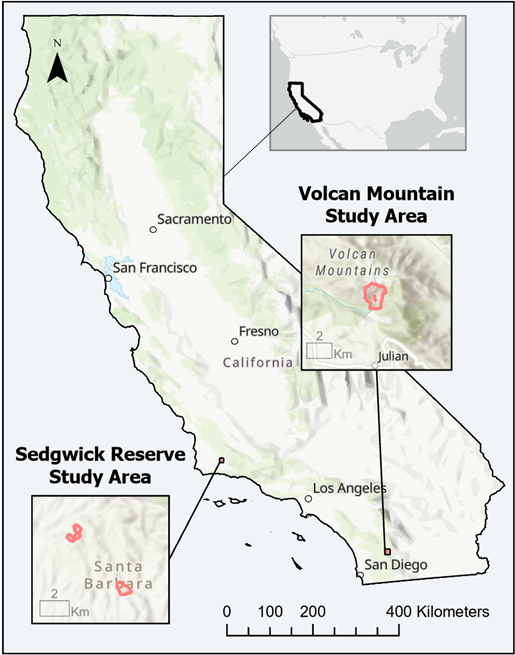
\includegraphics[width=0.65\linewidth]{manuscript/figures/Overall_Study_Areas_v2.png}
    \caption{Locations of the Southern California UAV LiDAR surveys—Sedgwick
           Reserve–Midland School in the Santa Ynez Valley and Volcan Mountain
           Wilderness Preserve in the Peninsular Range.}
  \label{fig:overall_study_area}
\end{figure}



\section{Materials and Methods}

% \begin{wrapfigure}[20]{r}{0.48\textwidth}
%   % \vspace{-38pt}
%   % \captionsetup{aboveskip=2pt, belowskip=0pt} % tighten caption gap
%   \centering
%   \includegraphics[trim=0mm 0mm 0mm 0mm, clip, width=\linewidth]
%                   {manuscript/figures/Overall_Study_Areas_v2.png}
%   \caption{Locations of the Southern California UAV LiDAR surveys—Sedgwick
%            Reserve–Midland School in the Santa Ynez Valley and Volcan Mountain
%            Wilderness Preserve in the Peninsular Range.}
%   \label{fig:overall_study_area}
% \end{wrapfigure}

% % 48 % wide, 20 text-lines tall, on the right
% \wrapL{0.48}{manuscript/figures/Overall_Study_Areas_v2.png}%
%       {Locations of the Southern California UAV LiDAR surveys—Sedgwick
%        Reserve–Midland School in the Santa Ynez Valley and Volcan Mountain
%        Wilderness Preserve in the Peninsular Range.}%
%       {fig:overall_study_area}

The core challenge addressed by this research is the enhancement of sparse and outdated national airborne LiDAR datasets. To train and validate supervised upsampling models, we collected dense UAV LiDAR as a benchmark of actual vegetation structure. The sections below describe the study areas where this data was collected, the multi-modal input data sources, and steps taken to ensure spatial alignment and consistency across all modalities.


\subsection{Study Area}


The study area (Figure \ref{fig:overall_study_area}) consists of two separate sites in Southern California, USA.
The first study area includes parts of the 24-square-kilometer Sedgwick Reserve, managed by the University of California, Santa Barbara, and the adjacent 11.5 square kilometer Midland School property. Both sit within the San Rafael Mountain foothills of Santa Barbara County (Figure \ref{fig:sedgwick_study_area}).


\begin{figure}%[!b]
  \centering
  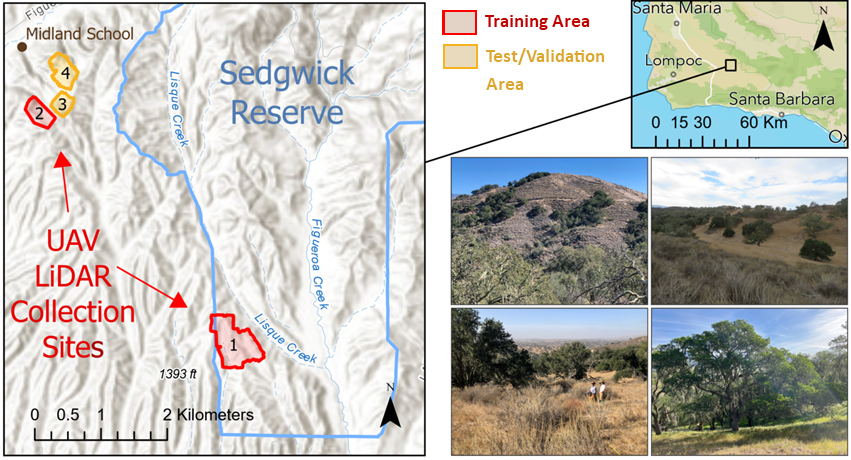
\includegraphics[width=1\linewidth]{manuscript/figures/Sedgwick_Reserve_Study_Area.png}
    \caption{The first study area combines parts of the Sedgwick Reserve and Midland School property in the San Rafael Mountain foothills, Santa Barbara County. It features diverse vegetation such as oak woodlands, chaparral, grasslands, and coastal sage scrub. Within this area, four UAV LiDAR sites were surveyed, covering a total of 70 hectares.}
  \label{fig:sedgwick_study_area}
\end{figure}

The area spans elevations from 287 to 852 meters and supports a mosaic of vegetation types with varying canopy architectures, including coastal sage scrub, native grasslands, chaparral (shrublands), coast live and blue oak woodlands, valley oak savanna, riparian habitats, and gray pine forests. UAV LiDAR was collected on four sites (totaling about 71 hectares) within the study area (Table \ref{tab:lidar_sites}). Given their similar terrain and vegetation, two sites were used for training, while the two smallest were withheld for independent model evaluation.


% % \vspace*{\fill} % push content down from above
% \begin{table}[H]
%   \centering
%   \caption{UAV LiDAR sites used as ground truth for model development}
%   \label{tab:lidar_sites}
%   \begin{tabular}{@{}cllll@{}}
%     \toprule
%     Site & Hectares & Location & Collection Date & Model Use\\ \midrule
%     1 & 38 & Sedgwick Reserve & 30 Jun 2023 & Training\\
%     2 & 12 & Midland School   & 23 Oct 2023 & Training \\
%     3 & 9 & Midland School & 23 Oct 2023 & Test/Validation\\
%     4 & 11 & Midland School   & 28 Sep 2023 & Test/Validation\\

%     5 & 197 & Volcan Mountain & 25 Oct 2024 & \begin{tabular}[c]{@{}l@{}}70\% Training\\ 30\% Test/Validation\end{tabular}\\
%     \bottomrule
%   \end{tabular}
% \end{table}
\begin{table}[H]
  \centering
  \caption{UAV LiDAR sites used as ground truth for model development}
  \label{tab:lidar_sites}
  \begin{tabular}{@{}cllll@{}}
    \toprule
    Site & Hectares & Location & Collection Date & Model Use \\ \midrule
    1 & 38  & Sedgwick Reserve & 30 Jun 2023 & Training \\
    2 & 12  & Midland School   & 23 Oct 2023 & Training \\
    3 &  9  & Midland School   & 23 Oct 2023 & Test/Validation \\
    4 & 11  & Midland School   & 28 Sep 2023 & Test/Validation \\
    5 & 197 & Volcan Mountain  & 25 Oct 2024 &
        \makecell[l]{70\% Training\\ 30\% Test/Validation} \\
    \bottomrule
  \end{tabular}
\end{table}

% \vspace*{\fill} % push content up from below
The second study area (Figure \ref{fig:volcan_mtn_study_area}) comprises 197 hectares within and adjacent to the Volcan Mountain Wilderness Preserve in the Peninsular Range of Southern California. The reserve is managed by San Diego County and the Volcan Mountain Foundation and ranges in elevation from about 1220 meters to over 1675 meters.
% \newpage
 It hosts diverse plant communities, including oak woodlands, chaparral, mixed conifer forests, and grasslands.  To ensure robust model evaluation across this ecological gradient, roughly 30 percent of the area (58 hectares) was reserved for testing and validation (Table \ref{tab:lidar_sites}). The three holdout zones (Figure \ref{fig:volcan_mtn_study_area}) used for model evaluation were selected to reflect the site’s vegetation diversity: the northernmost area includes chaparral that replaced forest following wildfires in 2003 and 2005; the central zone contains dense mixed-conifer and riparian vegetation interspersed with oak woodlands and chaparral; and the southernmost zone is predominantly semi-continuous oak canopy.

\begin{figure}[!t]
    \centering
    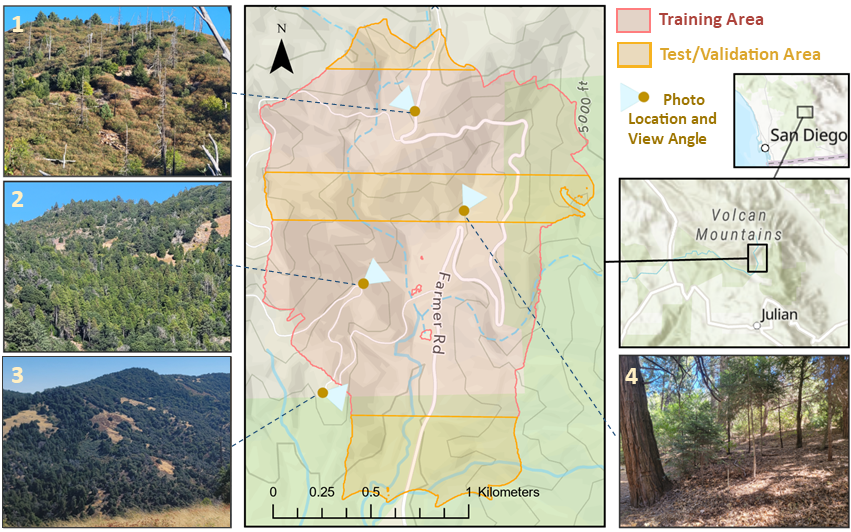
\includegraphics[width=1\linewidth]{manuscript/figures/Volcan_Mtn_Study_Area.png}
    \caption{Volcan Mountain study area (197 hectares) in the Peninsular Range of Southern California, encompassing diverse vegetation types across an elevation range of 1220 to 1675 meters. Thirty percent of the site (58 hectares) was set aside for testing/validation in three zones: post-fire chaparral in the north, mixed conifer and riparian vegetation with oak and chaparral in the center, and oak woodland with semi-continuous canopy in the south. }
    \label{fig:volcan_mtn_study_area}
\end{figure}






\subsection{The Data}

All remote‐sensing assets were co-registered within a common tiling framework covering both study sites.
First, the UAV‐LiDAR acquisition footprints were tessellated into 10 m × 10 m analysis tiles with 15\% overlap, yielding an initial set of 9,800 tiles at Sedgwick–Midland and 26,557 tiles at Volcan Mountain.  Each tile served as the spatial key for assembling a four-layer data stack (Table \ref{tab:data_summary})

% \begin{enumerate}[leftmargin=*]
%     \item \textbf{UAV LiDAR} point clouds (\textit{Sedgwick}-2023, 300 pts/m\textsuperscript{2}; \textit{Volcan}–2024, 300 pts/m\textsuperscript{2})
%     \item \textbf{3DEP airborne LiDAR} (\textit{Sedgwick}-2018, 22 pts/m\textsuperscript{2}; \textit{Volcan}-2015–16, 6 pts/m\textsuperscript{2})
%     \item \textbf{UAVSAR radar} coverage from 2014 to 2024 (6.17 m GSD)
%     \item \textbf{NAIP imagery} coverage from 2014 to 2022 (0.6–1 m GSD)
% \end{enumerate}

\begin{table}[H] % Using [H] from the float package to place it here.
\centering
\caption{Summary of remote sensing datasets used in the data stack.}
\label{tab:data_summary}
\begin{tabular}{l l p{4.5cm} l}
\toprule
\textbf{Data Source} & \textbf{Role in Study} & \textbf{Details} & \textbf{Revisit Rate} \\
\midrule
UAV LiDAR & Reference Data & $>$300 pts/m\textsuperscript{2} \newline \textit{Acquired: 2023--2024} & N/A \\
\addlinespace % Adds a little space between rows
3DEP Airborne LiDAR & Sparse Input & Sedgwick: $\sim$22 pts/m\textsuperscript{2} (2018) \newline Volcan: $\sim$6 pts/m\textsuperscript{2} (2015–16) & N/A \\
\addlinespace
UAVSAR (L-band) & Ancillary Input & 6.17 m GSD \newline \textit{Coverage: 2014--2024} & $\sim$2-3 years \\
\addlinespace
NAIP (Optical) & Ancillary Input & 0.6–1 m GSD \newline \textit{Coverage: 2014--2022} & $\sim$2 years \\
\bottomrule
\end{tabular}
\end{table}

By standardizing on overlapping 10 m patches, we guarantee that each training example draws from the same footprint across sensors—ensuring the model learns consistent, co-registered features from LiDAR, SAR, and imagery.

\subsubsection{UAV LiDAR Data}
\textit{Sedgwick and Midland Sites} - Between June and October 2023, UAV LiDAR data were collected by San Diego State Geography Department Staff on the Sedgwick and Midland School Sites using a DJI Matrice 300 drone equipped with a TrueView 515 LiDAR. The drone was flown at an altitude of approximately 60 meters above ground level, achieving a point density of around 300 points per square meter.

\textit{Volcan Mountain Site} - On October 25, 2024, the same Geography Department staff conducted flights using a  DJI Matrice 350 drone equipped with a TrueView 540 LIDAR system. This newer drone and sensor was flown at a higher altitude of approximately 110 meters above ground level, and still achieved a point density of over 600 points per square meter.

\subsubsection{Crewed Airborne LiDAR}
The available crewed airborne LiDAR (C-ALS) data includes two separate 3DEP datasets. The  Sedgwick  3DEP dataset, collected in 2018, has a point density of 22 pts/m\textsuperscript{2}. The C-ALS data for the Volcan Mountain site was collected between October 2015 and November 2016 and has a point density of 6.3 pts/m\textsuperscript{2} \citep{usgs_usgs_2016}. Both datasets were obtained from Microsoft's Planetary Computer \citep{us_geological_survey_3d_elevation_program_usgs_2023,planetary_computer}.
In addition to the point X, Y, and Z values we include three per-return attributes—intensity (16-bit integer 0–65,535 pulse magnitude), return number (ordinal of the return within its pulse), and number of returns (total returns from that pulse)—each standardized using the global mean and standard deviation computed across the full 3DEP dataset.

\begin{table}[H]
\centering
\caption{Timeline of NAIP and UAVSAR acquisitions for both study sites.}
\label{tab:imagery_timeline_v2}
\resizebox{\textwidth}{!}{% Make table fit within text width
\begin{tabular}{l cc cc}
\toprule
& \multicolumn{2}{c}{\textbf{Volcan Mountain}} & \multicolumn{2}{c}{\textbf{Sedgwick Reserve}} \\
\cmidrule(lr){2-3} \cmidrule(lr){4-5} % Creates partial rules under the merged cells
\textbf{Year} & \textbf{NAIP (GSD)} & \textbf{UAVSAR (\# Looks)} & \textbf{NAIP (GSD)} & \textbf{UAVSAR (\# Looks)} \\
\midrule
2014 & May (1 m) & Jun (3), Oct (2) & Jun (1 m) & Jun (8) \\
\addlinespace
2016 & Apr (60 cm) & --- & Jun (60 cm) & Apr (6) \\
\addlinespace
2018 & Aug (60 cm) & Oct (2) & Jul (60 cm) & --- \\
\addlinespace
2020 & Apr (60 cm) & --- & May (60 cm) & --- \\
\addlinespace
2021 & --- & Nov (2) & --- & --- \\
\addlinespace
2022 & Apr (60 cm) & --- & May (60 cm) & --- \\
\addlinespace
2023 & --- & --- & --- & Sep (6)\textsuperscript{a} \\
\addlinespace
2024 & --- & --- & --- & Oct (2) \\
\bottomrule
\multicolumn{5}{l}{\textsuperscript{a}\footnotesize{Part of the NASA FireSense initiative.}}
\end{tabular}%
}
\end{table}
\subsubsection{Synthetic Aperture Radar (SAR)}
Fully polarimetric L-band imagery (23.84 cm wavelength) from NASA’s UAVSAR system was obtained with the Alaska Satellite Facility’s \texttt{asf\_search} Python API \citep{alaska_search}.  The UAVSAR flights were conducted from a Gulfstream-III platform with bidirectional acquisitions from opposite look directions at an average altitude of 12,495 meters, providing multi-perspective radar coverage of the landscape at 6.17-meter ground resolution. We utilized six fully polarimetric multi-look cross-product channels: \texttt{HHHH}, \texttt{HVHV}, \texttt{VVVV}, \texttt{HHHV}, \texttt{HHVV}, and \texttt{HVVV}. The specific campaigns and acquisition details for each study site are summarized in Table \ref{tab:imagery_timeline_v2}. For every \SI{10}{m} × \SI{10}{m} 3DEP tile we extracted a co-centered \SI{20}{m} × \SI{20}{m} UAVSAR chip to accommodate layover and shadow extent, then bilinearly resampled each chip to \SI{5}{m} GSD before fusion with NAIP imagery and LiDAR.


\subsubsection{High-Resolution Aerial Imagery}
We ingested NAIP imagery through the Microsoft Planetary Computer STAC API \citep{planetary_computer} for survey years 2014–2022.
NAIP provides four-band (Red, Green, Blue, Near-Infrared) orthoimagery of the conterminous United States, collected at peak green-up on a two- to three-year cycle.  Prior to the 2016 flight season, data were delivered at 1 m ground-sample distance (GSD); since 2016 the native resolution has been 60 cm. A complete timeline of these acquisitions and their resolutions is provided in Table \ref{tab:imagery_timeline_v2}. For every 10 m × 10 m 3DEP tile we extracted a 20 m × 20 m NAIP chip centered on the same point to accommodate viewing-geometry variance and to capture neighboring shadows.  All NAIP scenes were then resampled to a common 50 cm grid.



\subsection{Data Cleaning and Preprocessing}
To reduce computational load and give the upsampling network a uniform-density target, we downsampled the UAV LiDAR for every tile with an adaptive anisotropic voxel grid. Each cloud was first voxelized at a 4 cm × 4 cm × 2 cm resolution; if more than 50,000 points remained, the horizontal voxel edge was incrementally enlarged (keeping the vertical edge at 50\% of that value) and the filter reapplied until the count fell below the limit. The resulting point sets preserve fine vertical structure while standardizing horizontal density.

To bound memory use and keep attention context sizes tractable, we cap the input 3DEP point cloud at $N_{\max}=10{,}000$ points per $10\times10$\,m tile. If a tile exceeds this count, we randomly subsample to $N_{\max}$ points; fewer than 1\% of tiles were affected. This cap defines the maximum attention sequence length and thus the model's memory footprint.

The dataset was partitioned into training, validation, and test sets using reference polygons to ensure the holdout sets captured the full environmental gradients found in the training data. During supervised training/evaluation, we applied quality thresholds—UAV to 3DEP point count ratio > 2 and at least 16,000 UAV LiDAR points and 200 3DEP points per tile—to exclude edge-of-flight tiles and extremely sparse cases, ensuring a meaningfully denser UAV reference and minimally informative 3DEP input for stable supervision. These thresholds served only as dataset curation filters and are not required at inference.

\subsection{Data Augmentation}
To increase the model's robustness and prevent overfitting, we expanded the training dataset from 24,000 to 40,000 tiles via data augmentation\cite{zhu2024advancements, shorten2019survey}. First, we preferentially selected source tiles for this process, prioritizing those with high structural complexity (z-variance) and large vegetation changes. Each selected source tile was then used to generate a new, augmented sample by applying a random combination of transformations. These included geometric operations (rotations and reflections) applied to all data layers, and point cloud-specific perturbations (random point removal and jittering) applied only to the input LiDAR data.


%%%%%%%%%%%%%%%%%%%%%%%%%%%%%%%%%%%%%%%%%%
\subsection{Model Architecture}
\label{sec:architecture}
Our multimodal upsampling framework transforms a sparse 3DEP point cloud, plus co-registered NAIP and UAVSAR image chips, into a denser 3-D point cloud (Fig.~\ref{fig:pipeline}).
The network is built around the \textbf{Local–Global Point Attention Block} (LG-PAB; §\ref{sec:lgpab}), which provides permutation‐invariant feature learning, optional feature-guided upsampling, and long-range geometric context.
Five macro–components are arranged in a feed-forward sequence:
(1) point feature extraction, (2) imagery encoding, (3) cross-attention fusion, (4) feature expansion and refinement, and (5) point decoding.

\begin{widefigure}
    %\vspace{-20pt}
    \centering
    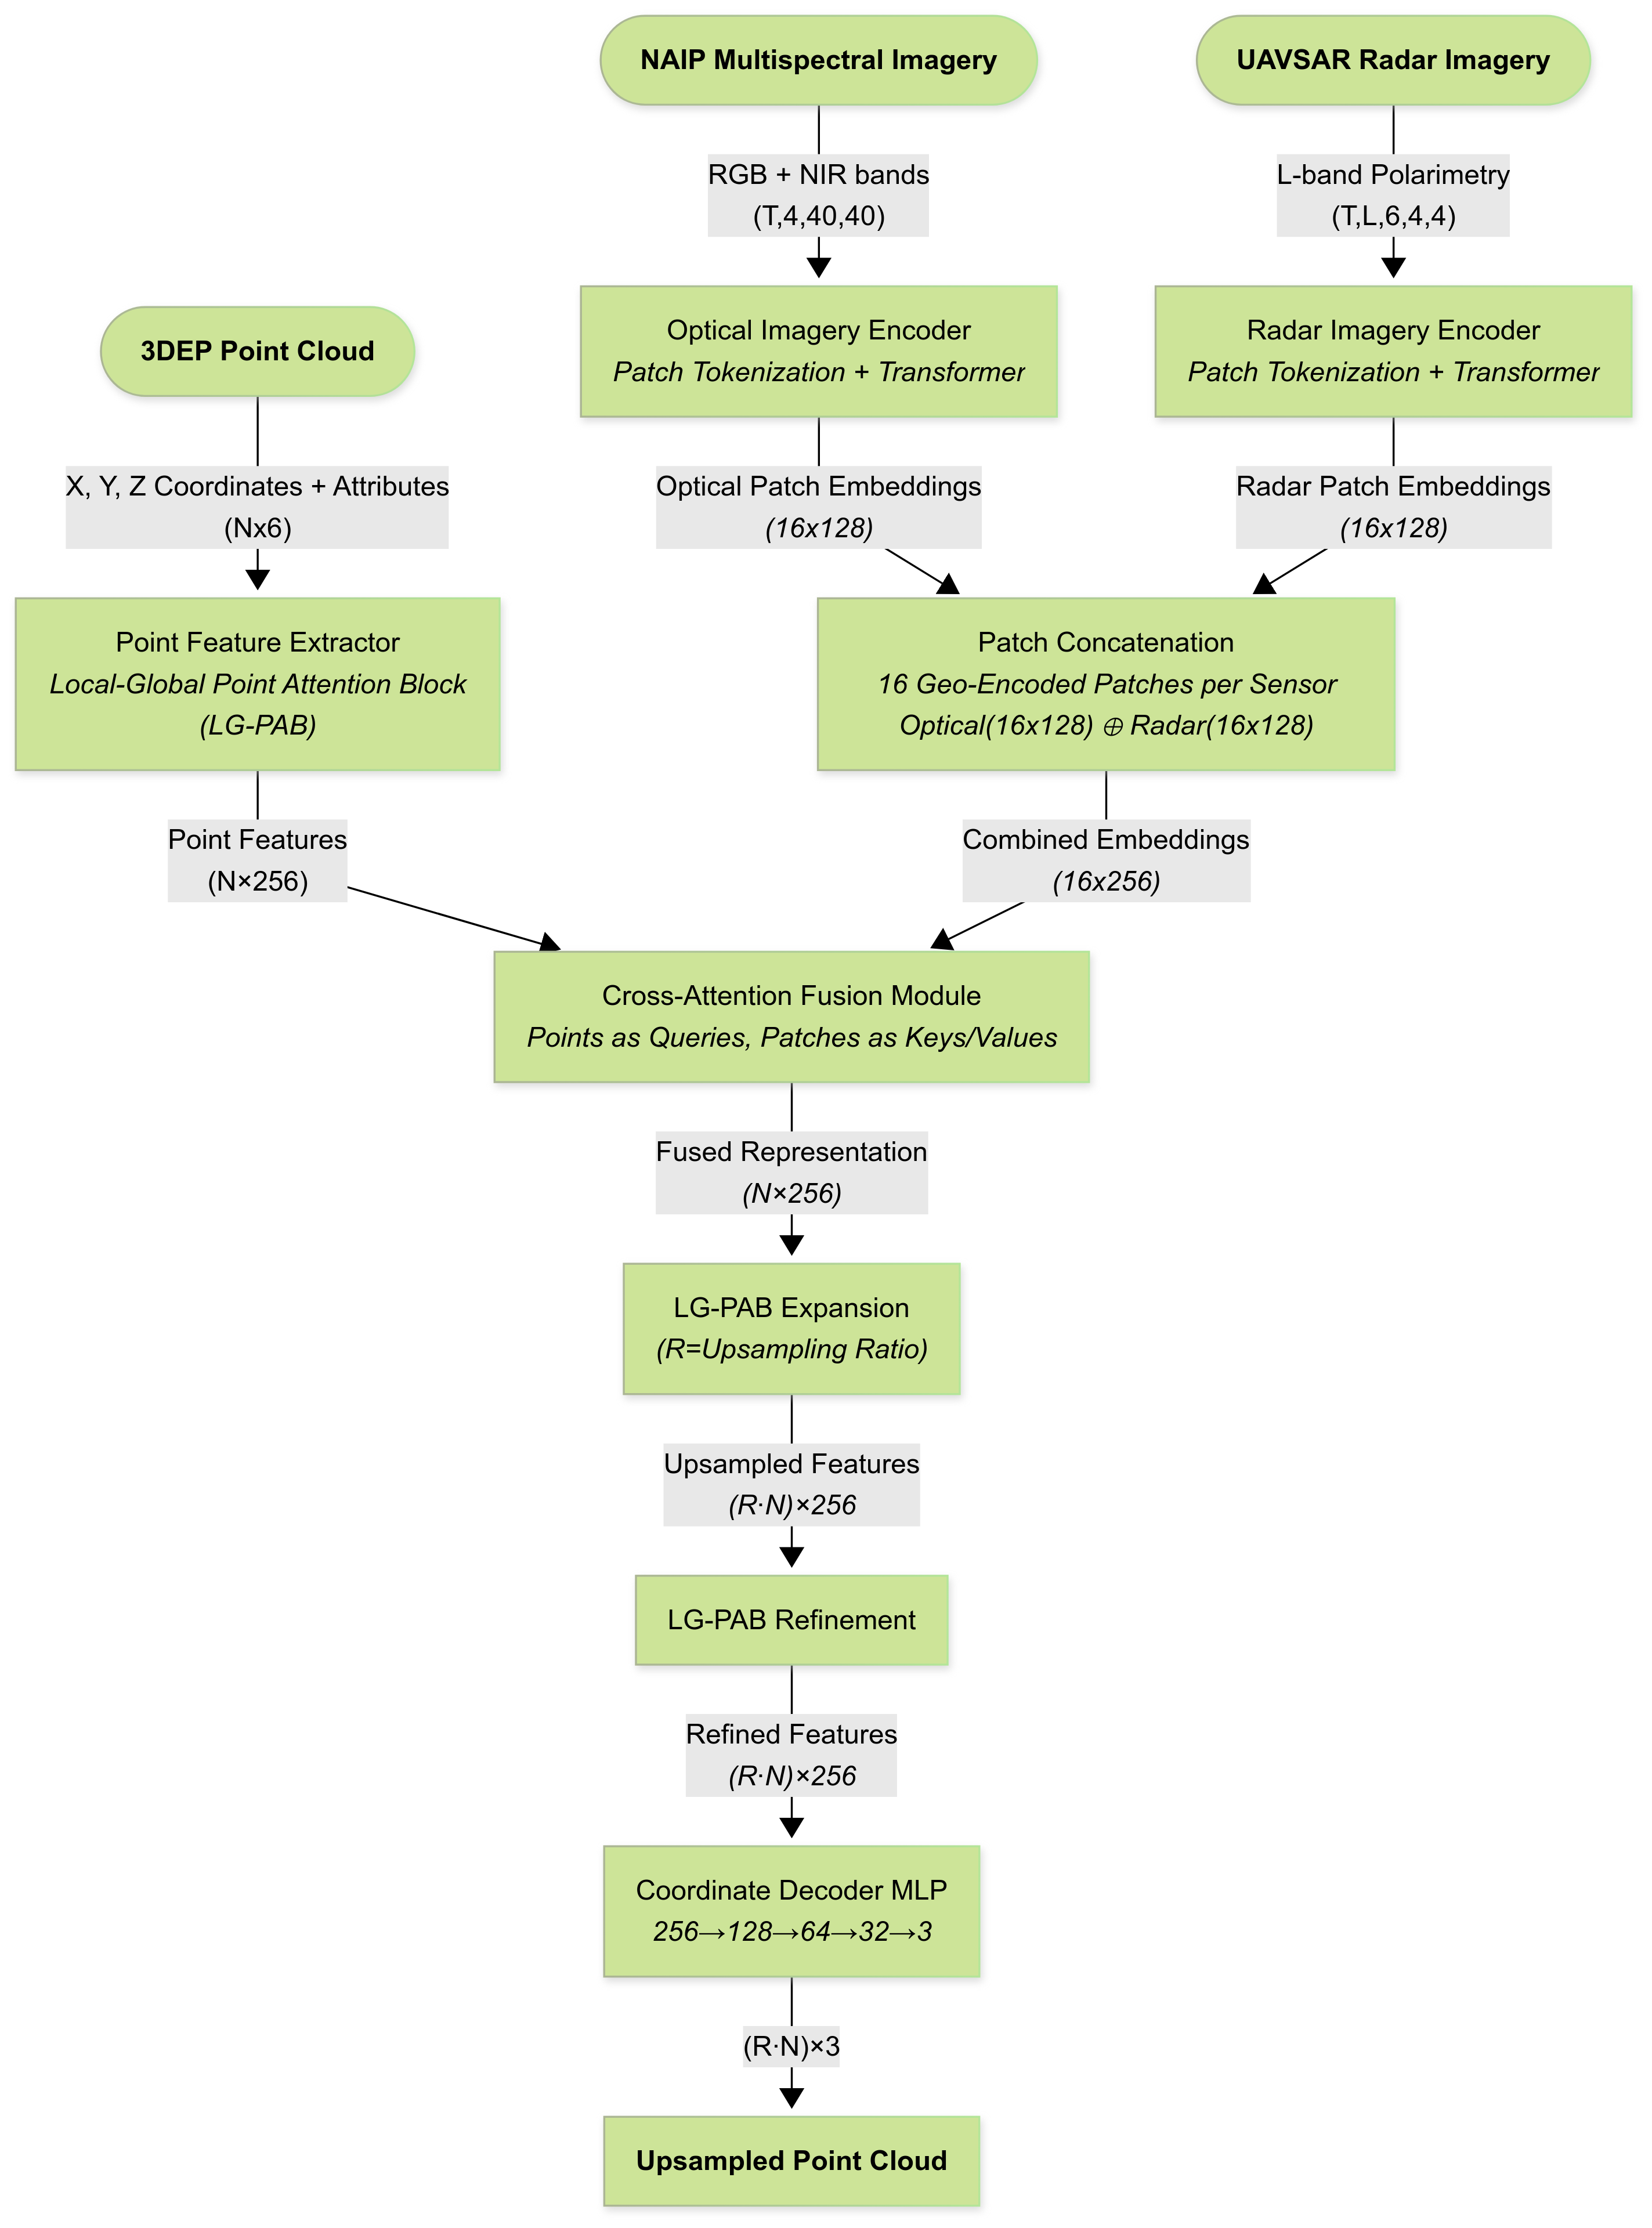
\includegraphics[trim=0mm 0mm 0mm 9mm, clip, width=1\linewidth]{manuscript/figures/Overall_Architecture.png}
    \caption{The overall multimodal upsampling architecture. Key components include Local–Global Point Attention Blocks, modality-specific imagery encoders for processing optical (NAIP) and radar (UAVSAR) data, and a cross-attention fusion module for combining imagery and LiDAR features.}
    \label{fig:pipeline}
\end{widefigure}




\paragraph{Notation Conventions}
Throughout this section, we use the following notation for tensor dimensions:
\begin{itemize}
    \item Counts: $N_{\text{pts}}$ (number of input points), $N_{\text{curr\_pts}}$ (current points in LG-PAB), $N_{\text{pts\_up}} = R_{\text{up}} \cdot N_{\text{pts}}$ (upsampled points), $N_{\text{patch}}$ (number of image patches, default 16), $N_{\text{time}}$ (temporal stack length), $N_{\text{looks}}$ (maximum look angles, $\leq 2$).
    \item Dimensions: $D_{\text{coord}} = 3$ (coordinate dimension), $D_{\text{attr}}$ (attribute dimension), $D_{\text{p\_feat}} = 256$ (point feature dimension), $D_{\text{p\_in}}$ (input point feature dimension), $D_{\text{p\_out}}$ (output point feature dimension), $D_{\text{token}} = 128$ (token dimension).
    \item Channels: $C_{\text{naip}} = 4$ (NAIP channels), $C_{\text{uavsar}} = 6$ (UAVSAR channels).
    \item Image dimensions: $H_{\text{naip}} = W_{\text{naip}} = 40$ (NAIP height/width), $H_{\text{uavsar\_pr}} = W_{\text{uavsar\_pr}} = 4$ (UAVSAR patch region height/width).
    \item Other: $R_{\text{up}}$ (upsampling ratio, default 2), $k_{\text{knn}} = 16$ (k-nearest neighbors).
\end{itemize}
For tensors, we use the notation TensorSymbol: (dim$_1$, dim$_2$, ..., dim$_k$) to describe their dimensions.

\noindent\textit{Figure notation bridge.} In Fig.~\ref{fig:lgpab} the generic diagram labels \texttt{in\_features} and \texttt{out\_features} (and the shortened \texttt{out\_feat} on two arrows) correspond to $D_{\text{p\_in}}$ and $D_{\text{p\_out}}$ in the above notation. (We used Mermaid for the schematic, which does not support mathematical subscripts, so plain text placeholders were used.)

Given an input cloud $P_{\text{in}}: (N_{\text{pts}}, D_{\text{coord}})$ with points $\{\mathbf{x}_i\}_{i=1}^{N_{\text{pts}}}\subset\mathbb{R}^{D_{\text{coord}}}$ and attributes $\mathbf{a}_i: (D_{\text{attr}})$, the network outputs $P_{\text{out}}: (N_{\text{pts\_up}}, D_{\text{coord}})$ with points $\{\hat{\mathbf{x}}_j\}_{j=1}^{N_{\text{pts\_up}}}$ where $N_{\text{pts\_up}} = R_{\text{up}} \cdot N_{\text{pts}}$ (typically $R_{\text{up}} = 2$).

An overview is:

\begin{enumerate}[leftmargin=*]
\item \textbf{LG-PAB Extractor} $\;\mathcal{E}_{\mathrm{pt}}$
      $\;\rightarrow$ local–global point features $F: (N_{\text{pts}}, D_{\text{p\_feat}})$;
\item \textbf{Imagery Encoders} $\;\mathcal{E}_{\mathrm{opt}},\mathcal{E}_{\mathrm{rad}}$
      $\;\rightarrow$ NAIP and UAVSAR patch embeddings $E_{\text{opt}}, E_{\text{rad}}: (N_{\text{patch}}, D_{\text{token}})$;
\item \textbf{Cross-Attention Fusion} $\;\mathcal{F}_{\mathrm{ca}}$
      $\;\rightarrow$ enriched point features $F_{\!\mathrm{fused}}: (N_{\text{pts}}, D_{\text{p\_feat}})$;
\item \textbf{LG-PAB Expansion \& Refinement}
      $\;\rightarrow$ upsampled features $F^{\uparrow}: (N_{\text{pts\_up}}, D_{\text{p\_feat}})$ and coordinates $P^{\uparrow}: (N_{\text{pts\_up}}, D_{\text{coord}})$;
\item \textbf{MLP Decoder} $\;\rightarrow$ residual offsets $\Delta P: (N_{\text{pts\_up}}, D_{\text{coord}})$ and final coordinates $P_{\mathrm{out}}: (N_{\text{pts\_up}}, D_{\text{coord}})$.
\end{enumerate}

\paragraph{Complexity, memory, and sequence length across stages.}
Global multi-head attention remains quadratic in the number of points within a tile. The 10\,m tiling and the input cap $N_{\max}=10{,}000$ fix the extractor’s attention sequence length; with the feature-guided expansion set to $R_{\text{up}}=2$, the largest sequence arises immediately after expansion and is at most $\approx 2\times N_{\text{pts}} \le 20{,}000$ before refinement and decoding. We implement global attention with FlashAttention, which reduces memory traffic while preserving exact attention. Under these bounds, we observed stable runtime and memory without requiring additional approximations or pruning.

% --- LG-PAB (its own page) ---------------------------------------------------
% \clearpage
\subsection{The Local–Global Point Attention Block (LG-PAB)}
\label{sec:lgpab}

% \begin{wrapfigure}[40]{r}{0.43\textwidth}
\begin{figure}[!b]
  \centering
  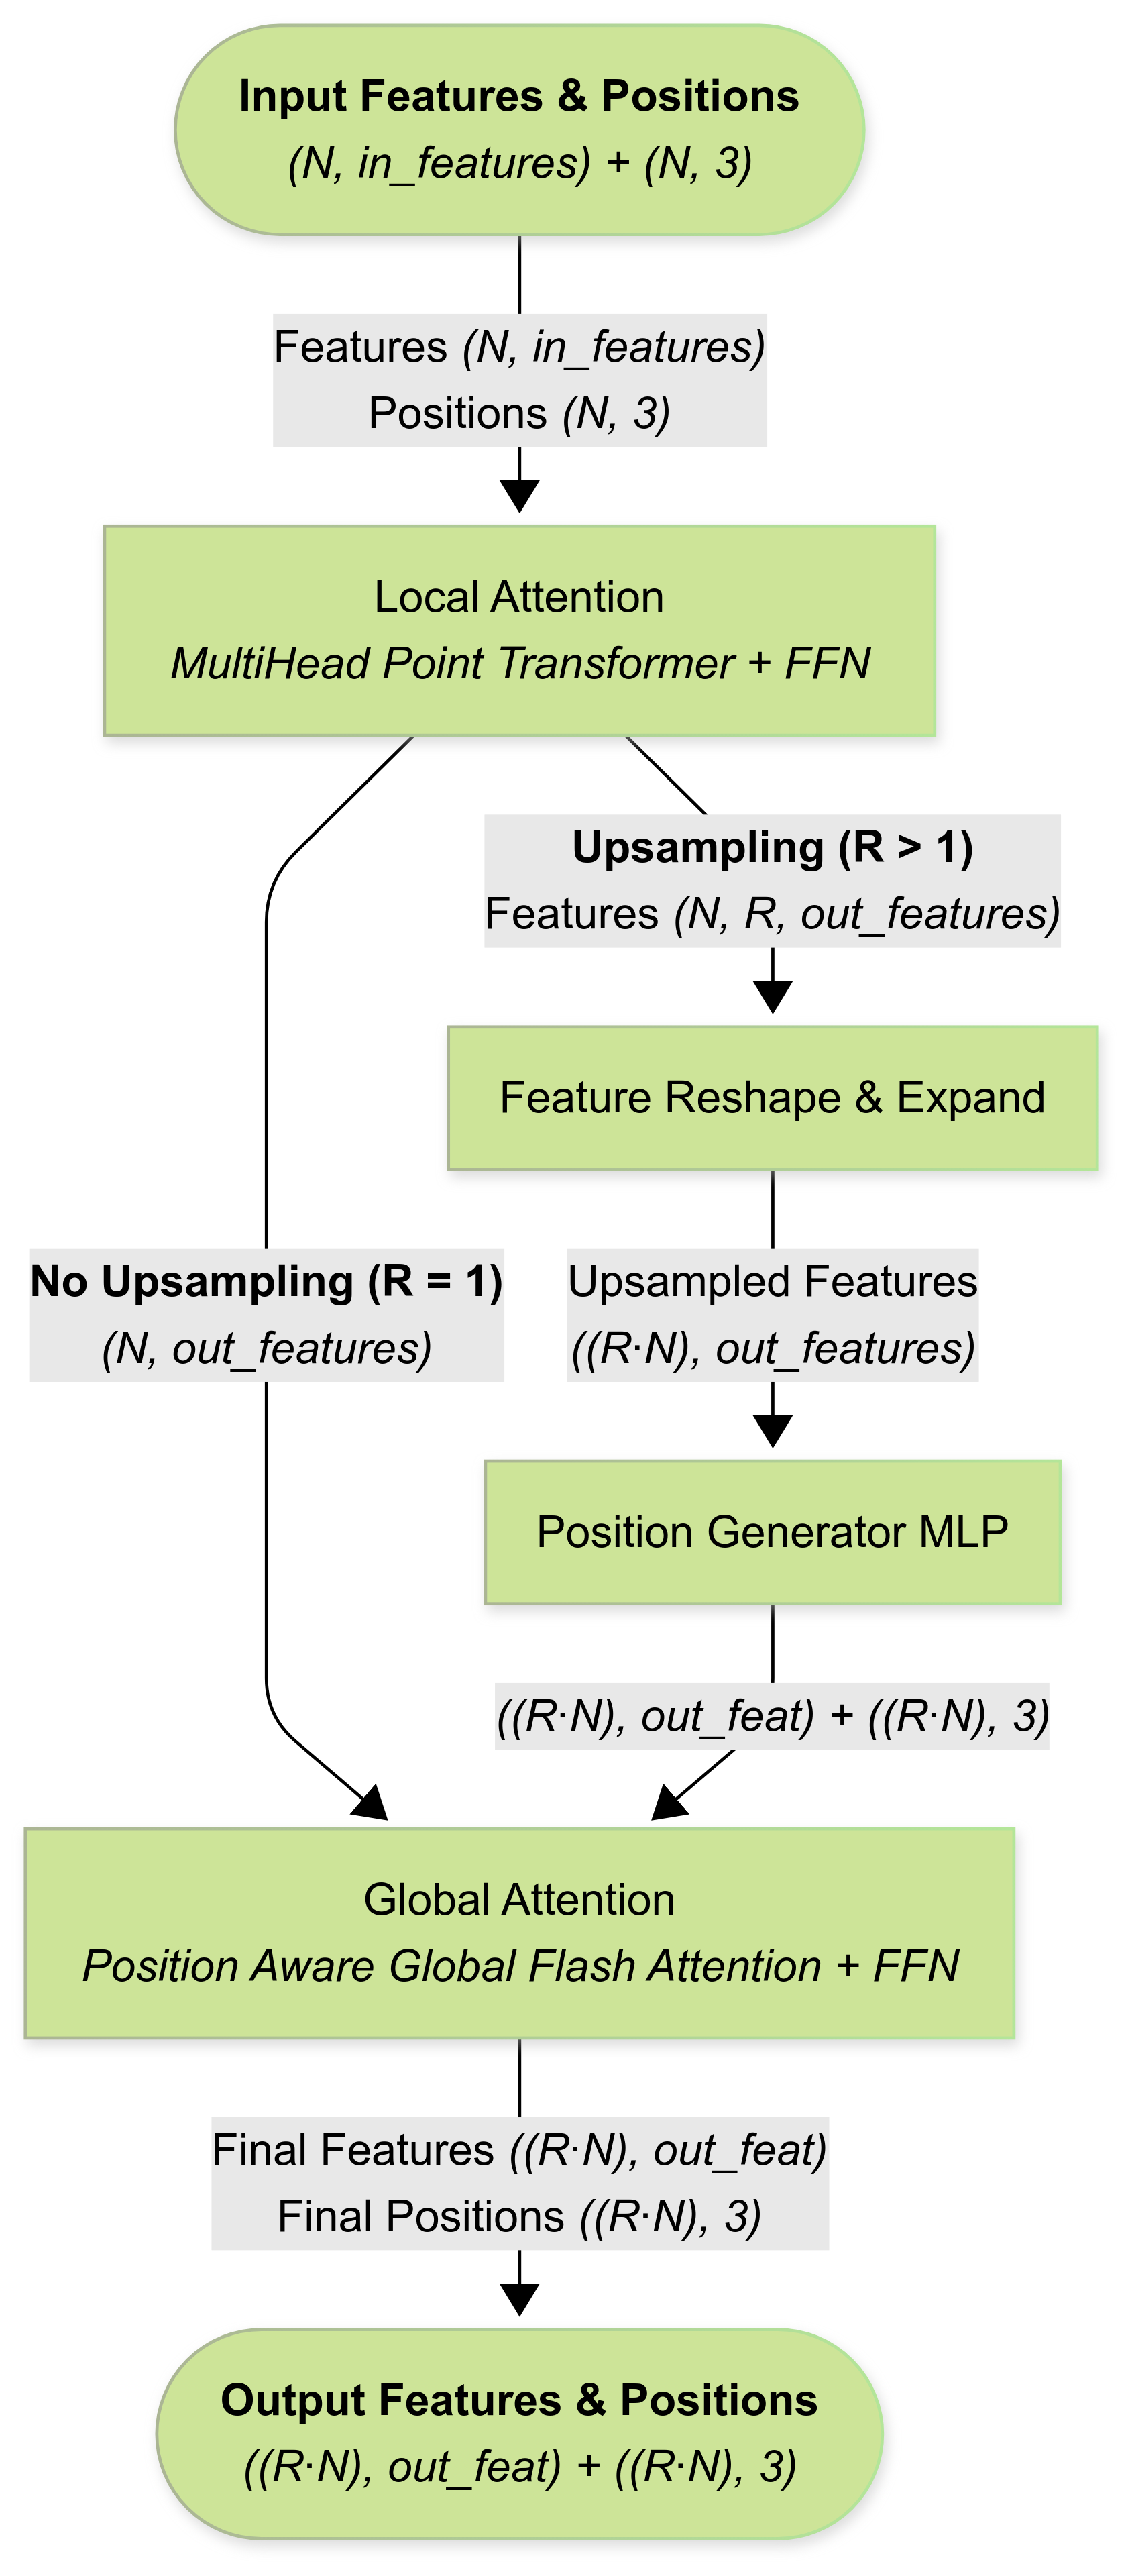
\includegraphics[trim=0mm 0mm 36mm 0mm, clip, width=0.5\textwidth]{manuscript/figures/LG-PAB.png}
  \caption{Flowchart of the Local–Global Point Attention Block (LG-PAB), the core computational unit used across the feature extraction, expansion, and refinement stages. The block applies local attention via a multi-head Point Transformer, optional upsampling with learned position offsets, and global multi-head Flash Attention for broader spatial context. A feed-forward MLP follows both the local and global attention blocks.}
  \label{fig:lgpab}
\end{figure}
% \end{wrapfigure}%

Figure~\ref{fig:lgpab} presents a flow-chart of the \emph{Local–Global Point Attention Block}, the fundamental unit used three times in our architecture (extraction, expansion, and refinement stages).
Each LG-PAB converts an input tuple $\langle X, P \rangle$ consisting of point features $X: (N_{\text{curr\_pts}}, D_{\text{p\_in}})$ and 3-D coordinates $P: (N_{\text{curr\_pts}}, D_{\text{coord}})$ into refined (and optionally upsampled) features and positions. The block proceeds through the stages that appear in the diagram:

\begin{enumerate}[leftmargin=*]
\item \textbf{Local Attention Block}
      A \textsc{Multi-Head Point Transformer} operates on a $k_{\text{knn}}$-nearest-neighbour graph ($k_{\text{knn}}{=}16$) to capture fine-scale geometry. Its output passes through a two-layer \textsc{Feed-Forward Network} (FFN) with GELU activation, producing an intermediate tensor
      $Z: (N_{\text{curr\_pts}}, R_{\text{up}} \cdot D_{\text{p\_out}})$.
      When the upsampling ratio $R_{\text{up}}{=}1$ this step already delivers the final per-point features.

\item[\emph{2\,a}] \textbf{Feature-Guided Upsampling (optional)}
      If $R_{\text{up}}{>}1$ (expansion stage) the intermediate tensor is reshaped to $[N_{\text{curr\_pts}}, R_{\text{up}}, D_{\text{p\_out}}]$, effectively cloning each feature vector $R_{\text{up}}$ times.
      A small \textbf{Position-Generator MLP} then predicts a 3-D offset for every clone, yielding new coordinates
      $\hat{P} = P^{\text{rep}} + \Delta P: (N_{\text{curr\_pts}} \cdot R_{\text{up}}, D_{\text{coord}})$.
      The features are flattened back to $[N_{\text{curr\_pts}} \cdot R_{\text{up}}, D_{\text{p\_out}}]$.

\item \textbf{Global Attention Block}
      To impose long-range coherence, the upsampled (or original) features are processed by \textsc{Position-Aware Global Flash Attention}. Coordinates are first embedded by a two-layer MLP, concatenated to the features, and fed to a four-head FlashAttention layer that attends across \emph{all} points in the tile. A second FFN refines the attended features, after which residual connections and LayerNorm complete the block.
\end{enumerate}

% --- Imagery Encoders (its own page) ----------------------------------------
% \clearpage
\subsection{Imagery Encoders}
\label{sec:img_enc}

% \begin{wrapfigure}[20]{r}{0.45\textwidth}
%   \vspace{-25pt}
%   \centering
%   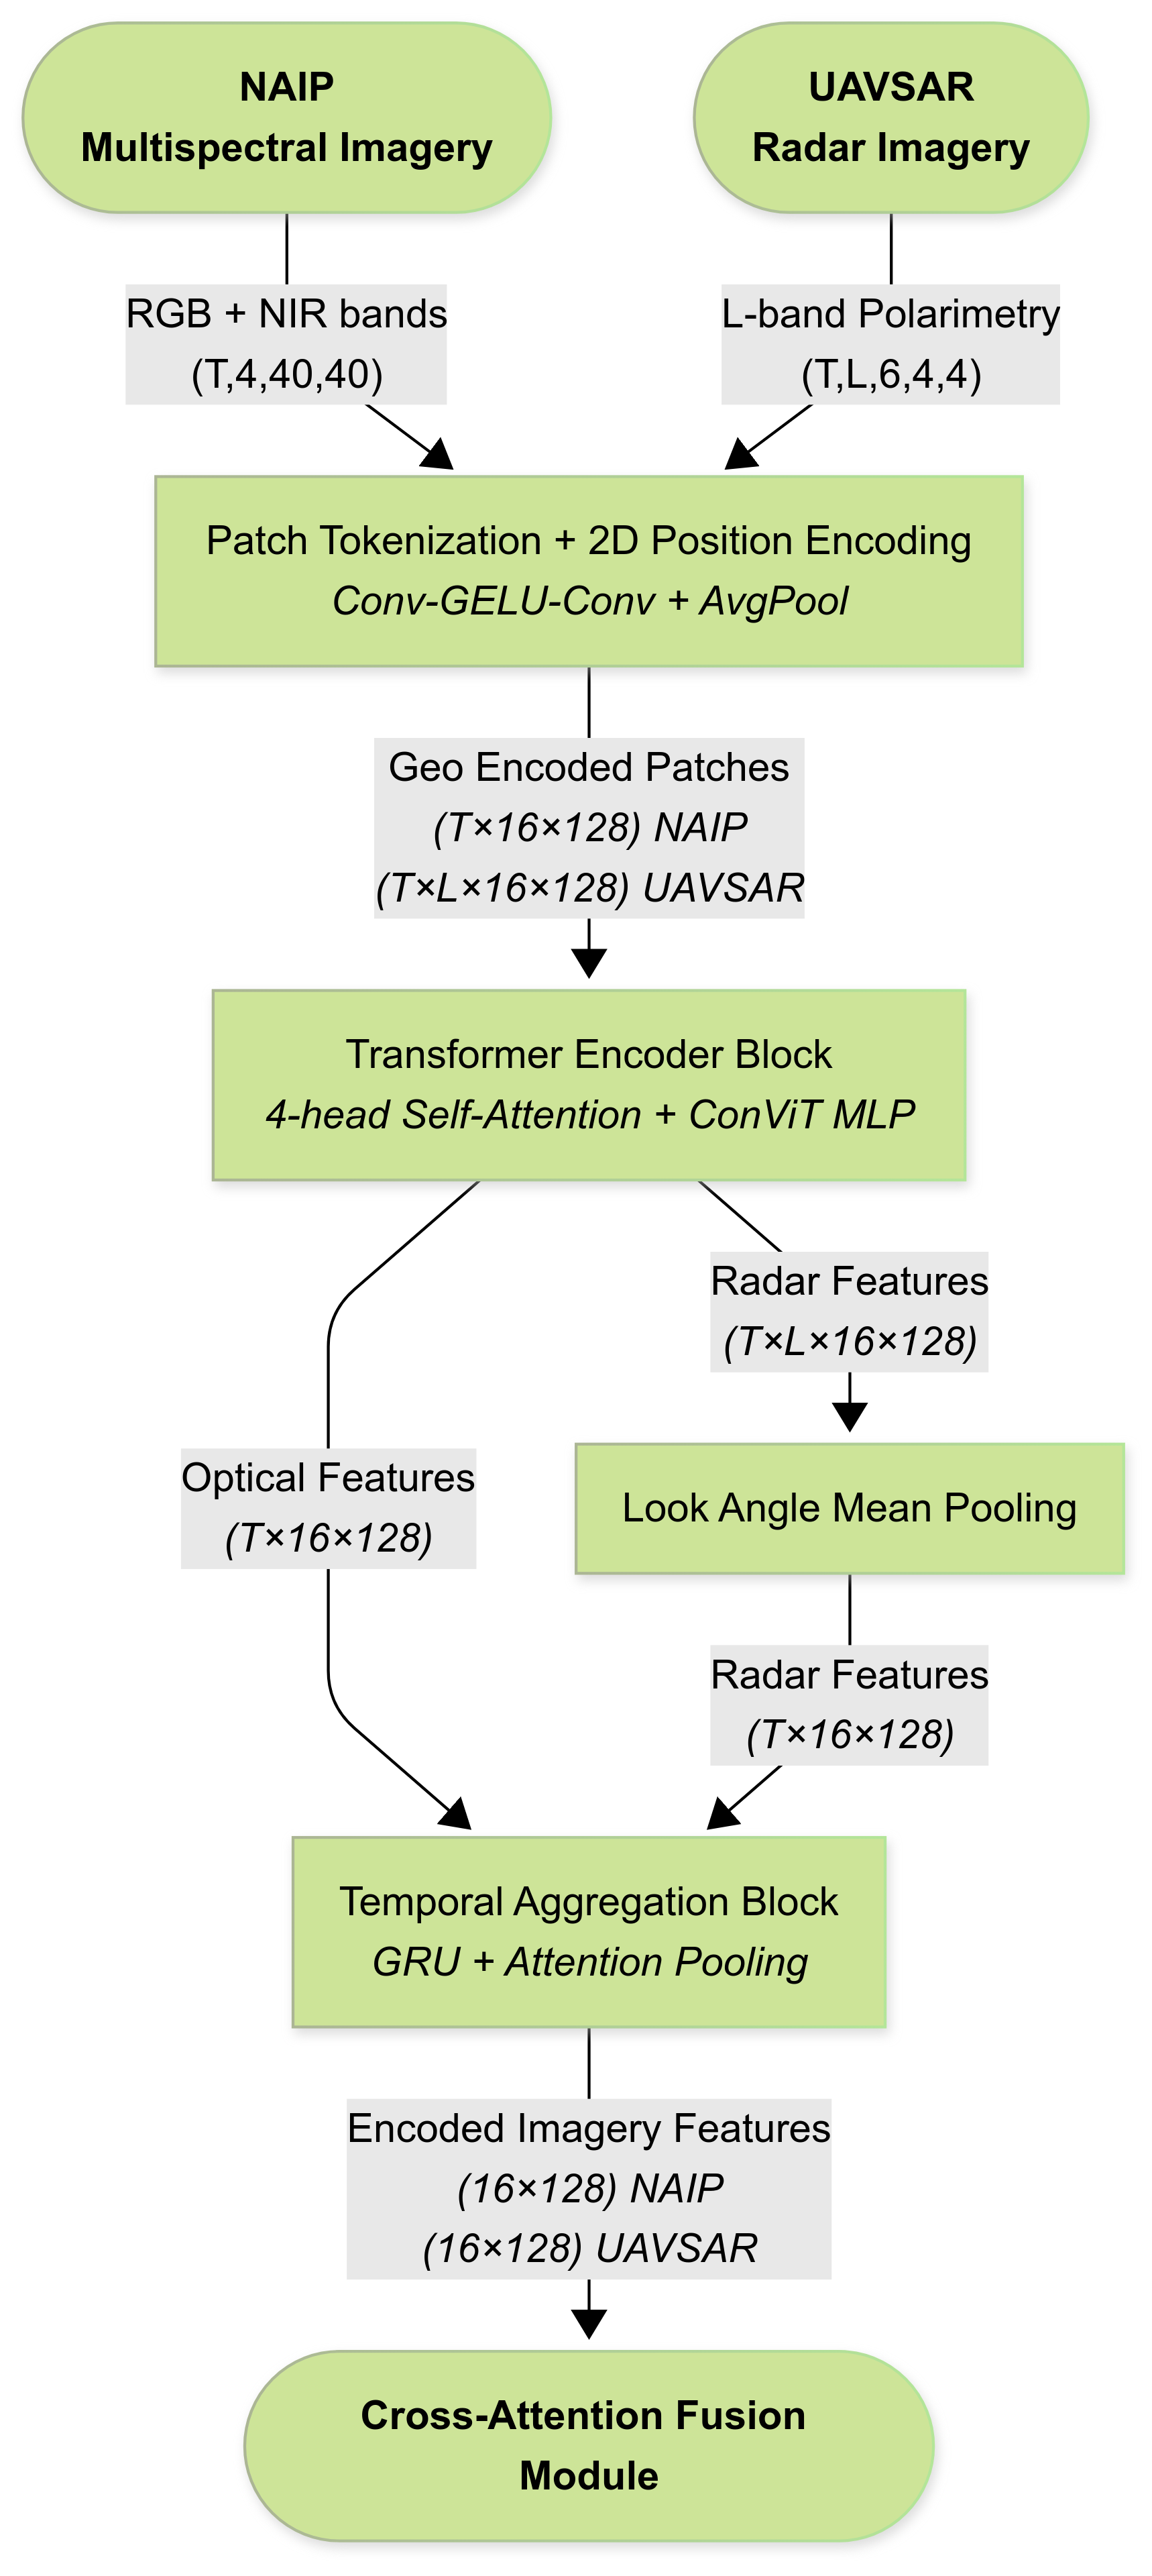
\includegraphics[trim=0mm 0mm 20mm 0mm, clip, width=0.43\textwidth]{manuscript/figures/Imagery_Encoders.png}
%   \caption{Architecture diagram of the imagery encoders. Image stacks from NAIP (optical) and UAVSAR (radar) pass sequentially through Patch Tokenization, Transformer Encoder blocks for spatial context modeling, and a Temporal GRU-Attention Head for temporal aggregation.}
%   \label{fig:imgenc}
% \end{wrapfigure}%

\begin{figure}
    %\vspace{-20pt}
    \centering
    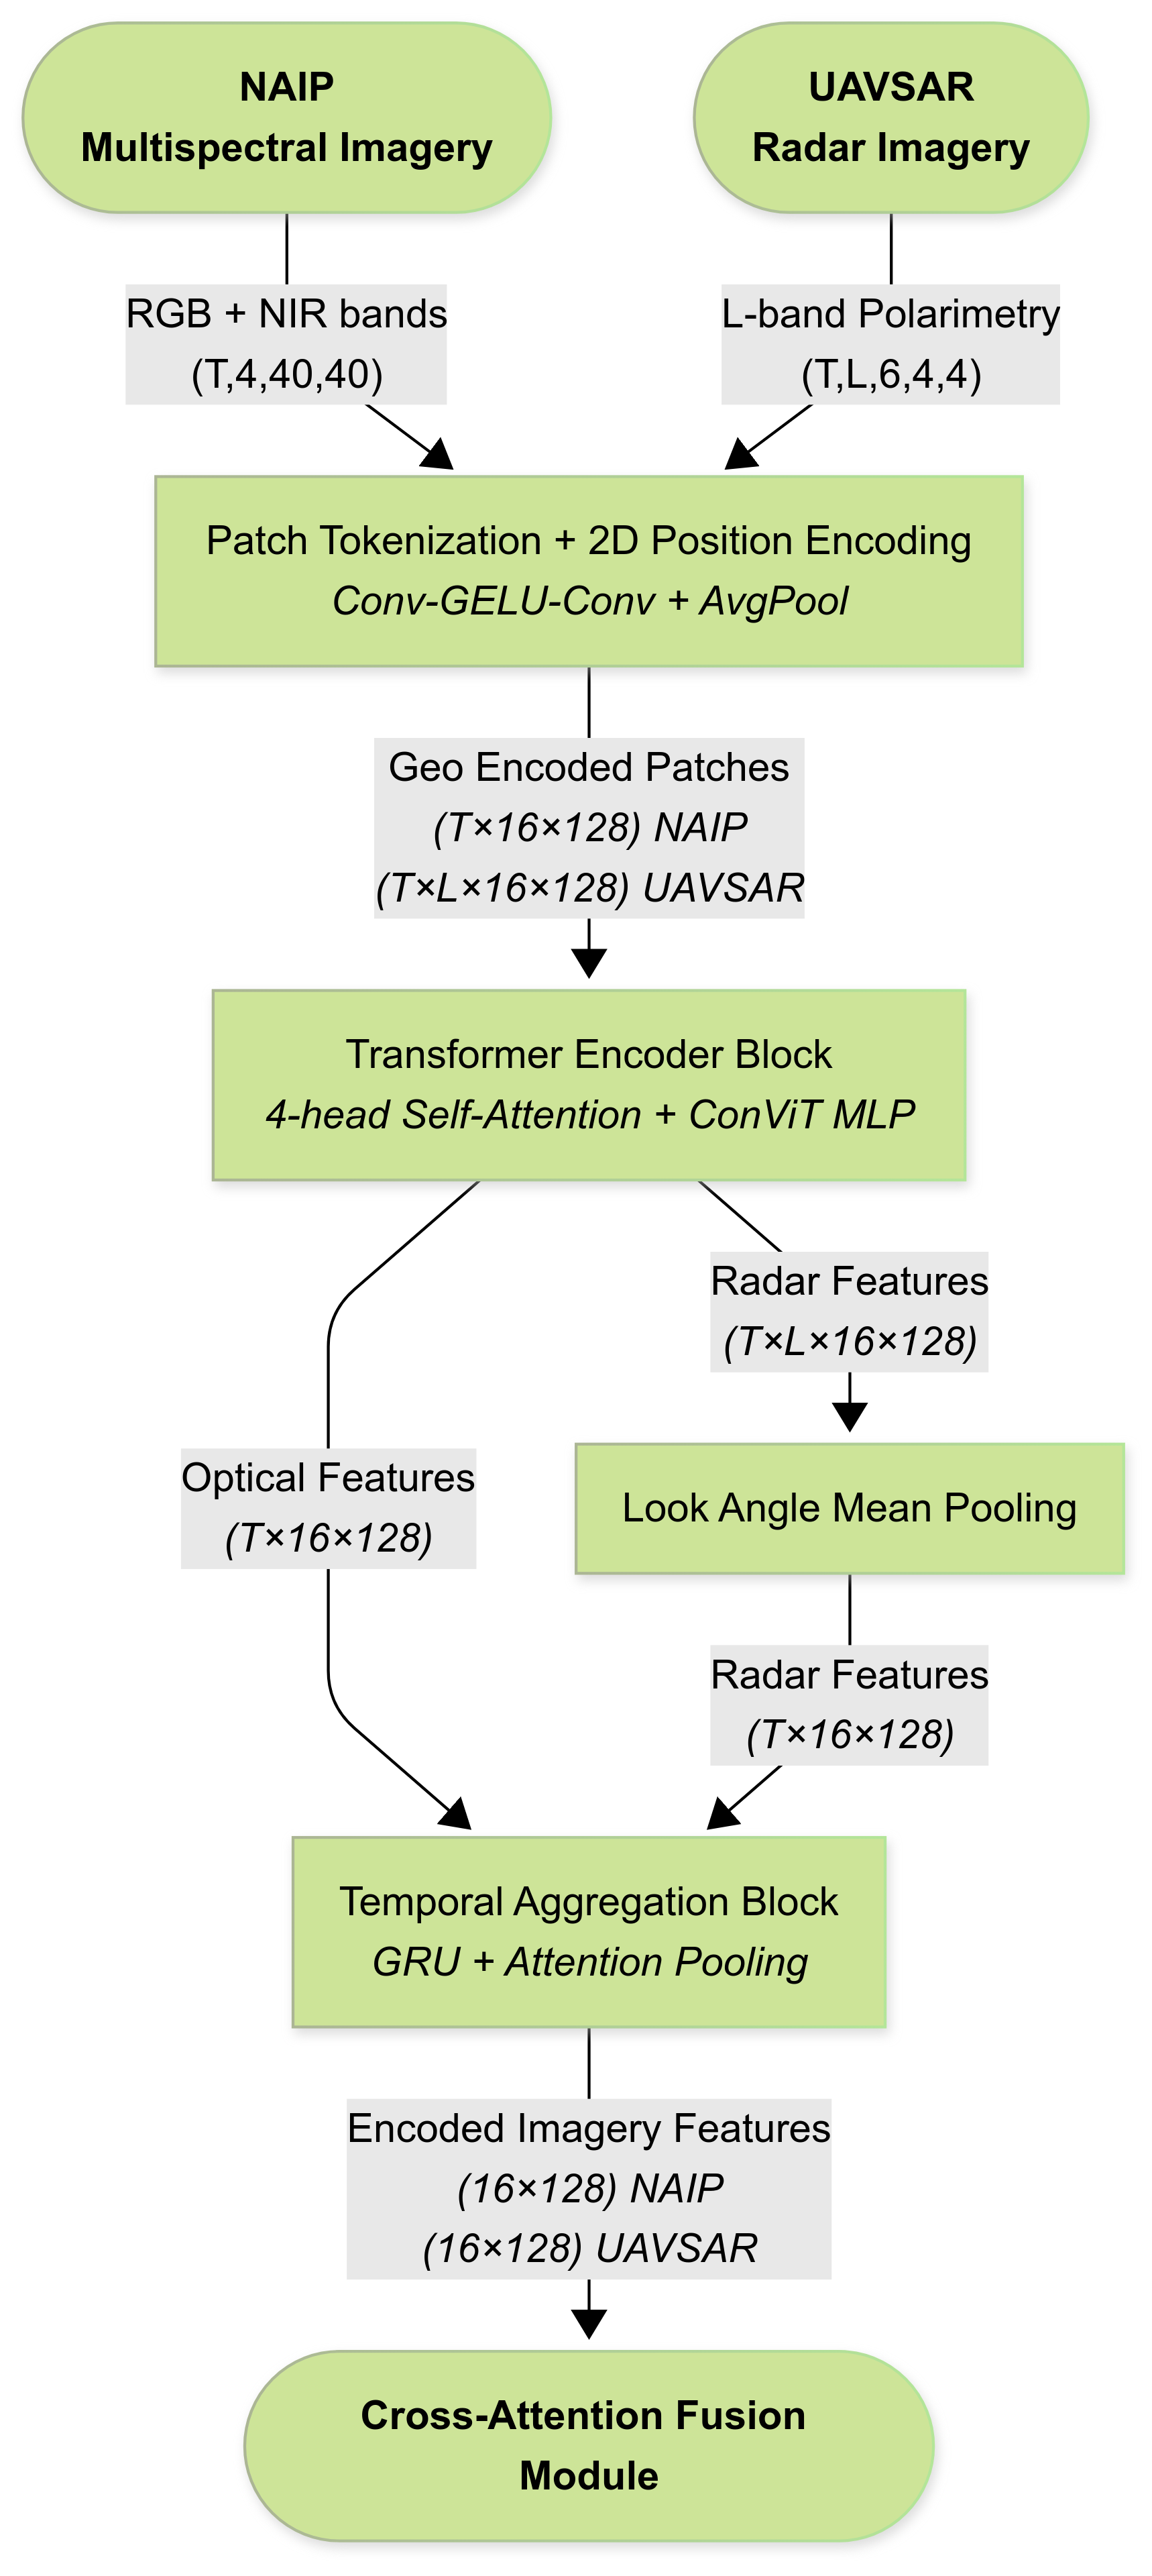
\includegraphics[trim=0mm 0mm 20mm 0mm, clip, width=0.7\linewidth]{manuscript/figures/Imagery_Encoders.png}
    \caption{Architecture diagram of the imagery encoders. Image stacks from NAIP (optical) and UAVSAR (radar) pass sequentially through Patch Tokenization, Transformer Encoder blocks for spatial context modeling, and a Temporal GRU-Attention Head for temporal aggregation.}
    \label{fig:imgenc}
\end{figure}

Optical (NAIP) and radar (UAVSAR) image chips are processed by a \emph{shared five-stage encoder} (with modality specific weights) that converts each image stack into a fixed set of patch tokens. The encoder stages—illustrated in Fig.~\ref{fig:imgenc}—are:

\begin{enumerate}[leftmargin=*]
\item \textbf{Patch Tokenization.}
      A two-layer Conv–GELU–Conv stem with stride-1 followed by average pooling (stride=$\texttt{patch\_size}$) extracts features on a $4\times4$ grid.
      This design mirrors Shifted Patch Tokenization, which adds local texture bias to Vision Transformers (ViTs) and improves sample efficiency on small datasets \cite{lee2021vision}.
  (Conv1: $C_{in}\rightarrow D_{\text{token}}/2$, $3\times3$, stride 1, pad 1; Conv2: $D_{\text{token}}/2\rightarrow D_{\text{token}}$, $3\times3$, stride 1, pad 1; AvgPool: kernel=stride=$\texttt{patch\_size}=10$.) The $N_{\text{patch}}=16$ patches are flattened to $Z_{\text{tok}}: (N_{\text{patch}}, D_{\text{token}})$ and normalized via LayerNorm.


\item \textbf{2-D Positional Encoding.}
      Normalized patch centers are embedded via a two-layer MLP and added to the tokens:
      $Z_{\text{pos}} = Z_{\text{tok}} + \text{MLP}_{\text{pos}}(x,y)$.

\item \textbf{Transformer Encoder Block.}
      A 4-head self-attention layer is paired with LayerScale ($\gamma \approx 10^{-5}$), a learnable scalar that stabilizes deep transformers \cite{touvron2021going}.
      The accompanying MLP includes a depth-wise 1-D convolution, following the ConViT approach to introduce a soft convolutional inductive bias \cite{dascoli2021convit}.
  MLP: $D_{\text{token}} \rightarrow 4 D_{\text{token}}$ (depth-wise 1-D conv $k=3$) $\rightarrow D_{\text{token}}$. The block outputs $Z_{\text{enc}}: (N_{\text{patch}}, D_{\text{token}})$.


\item \textbf{Temporal GRU–Attention Head.}
      For inputs with temporal length $N_{\text{time}}$, a bidirectional Gated Recurrent Unit (GRU) with attention pooling aggregates tokens into patch descriptors $E_{\text{patch}}: (N_{\text{patch}}, D_{\text{token}})$.
\end{enumerate}

Full per-component layer specifications (including fusion projections, LG-PAB FFNs, upsampling position generator, and coordinate decoder) appear in Appendix Table~\ref{tab:layer_specs} for transparency and reproducibility.

\paragraph{UAVSAR Look Angle Mean Pooling}
\begin{itemize}[leftmargin=*]
\item \textbf{UAVSAR.}
      Input $I_{\text{uavsar}}: (N_{\text{time}}, N_{\text{looks}}, C_{\text{uavsar}}, H_{\text{uavsar\_pr}}, W_{\text{uavsar\_pr}})$ with $N_{\text{looks}} \leq 2$.
      After the Transformer Encoder Block, we average features across available look angles to produce $Z_{\text{avg}}: (N_{\text{time}}, N_{\text{patch}}, D_{\text{token}})$ before temporal processing.
      Otherwise, the pipeline matches NAIP.
\end{itemize}


Both encoders output token matrices $E_{\text{opt}}$ and $E_{\text{rad}}: (N_{\text{patch}}, D_{\text{token}})$ that are normalized and concatenated before fusion.



\subsection{End-to-End Upsampling Pipeline}
\label{sec:pipeline}

\paragraph{1) Local–Global Feature Extraction.}
The sparse 3DEP cloud—concatenated with intensity, return number, and number of returns (6 attributes total)—is processed by the first \emph{Local–Global Point Attention Block} (§\ref{sec:lgpab}). The output is a set of point features $F: (N_{\text{pts}}, D_{\text{p\_feat}})$ that encode both neighborhood morphology and tile-level context.

\paragraph{2) Imagery Encoders.}
Co-registered NAIP and UAVSAR chips are independently tokenized and fed to lightweight Transformer encoders ($N_{\text{patch}}$ patches, embed dim $D_{\text{token}}$).
The optical encoder (RGB+NIR) outputs patch embeddings $E_{\text{opt}}: (N_{\text{patch}}, D_{\text{token}})$, whereas the radar encoder (L-band polarimetry) outputs $E_{\text{rad}}: (N_{\text{patch}}, D_{\text{token}})$.
When multiple acquisition dates exist, per-modality tokens are fused temporally via a shared GRU–attention head.

\paragraph{3) Cross-Attention Fusion.}
Point features act as \emph{queries} and image patches as \emph{keys/values} in a four-head cross-attention block.
Scaled dot-product scores are masked for patches whose centroid is more than 8 meters from the query point.
The fused representation $F_{\text{fused}}: (N_{\text{pts}}, D_{\text{p\_feat}})$ augments every point with spectral texture and volumetric back-scatter cues, improving discrimination of canopy surfaces versus gaps.

\paragraph{4) Feature-Guided Upsampling.}
A second LG-PAB with ratio $R_{\text{up}}=2$ expands $F_{\text{fused}}$ and predicts offsets $\Delta P$ that generate $N_{\text{pts\_up}}$ candidate coordinates. This stage doubles point density while maintaining local topology.

\paragraph{5) Feature Refinement.}
A third LG-PAB (ratio $R_{\text{up}}=1$) re-computes local and global attention on the enlarged cloud, ironing out artifacts introduced during expansion and propagating context across newly formed neighborhoods.

\paragraph{6) Coordinate Decoding.}
Finally, a four-layer MLP ($D_{\text{p\_feat}} \rightarrow 128 \rightarrow 64 \rightarrow 32 \rightarrow D_{\text{coord}}$) regresses residual offsets that are added to the upsampled positions, producing the higher-resolution prediction $\hat{P}: (N_{\text{pts\_up}}, D_{\text{coord}})$.

%-------------------------------------------------
\subsection{Training Protocol and Analysis}
\label{sec:study_design}
%-------------------------------------------------
To systematically evaluate our research questions, we established a rigorous training and analysis protocol. The full dataset, comprising tiles from both study areas, was partitioned into training, validation, and testing subsets. The training set consists of 24,000 original tiles, which was expanded to 40,000 through the data augmentation process described previously. A separate set of 3,792 tiles was reserved for validation during training, and a final hold-out set of 5,688 tiles was used for testing and performance evaluation (Table \ref{tab:data_prep}).
%---------------------------------------------------------------
% 1) Dataset preparation
%---------------------------------------------------------------
\begin{table}[htbp]
  \centering
  \caption{Dataset preparation}
  \label{tab:data_prep}
  \begin{tabular}{lr}
    \toprule
    \textbf{Subset} & \textbf{Tiles} \\
    \midrule
    Training        & 24\,000 original $+$ 16\,000 augmented $=$ 40\,000 \\
    Validation      & 3\,792 \\
    Test            & 5\,688 \\
    \bottomrule
  \end{tabular}
\end{table}

To isolate the impact of each data modality, we trained four distinct model variants (Table \ref{tab:model_variants}). A baseline model was trained using only the sparse 3DEP LiDAR input. Two single-modality models were trained by fusing the LiDAR with either NAIP optical imagery or UAVSAR radar data. Finally, a fully fused model was trained using all three data sources simultaneously.
%---------------------------------------------------------------
% 2) Model variants
%---------------------------------------------------------------
\begin{table}[htbp]
  \centering
  \caption{Model variants evaluated\footnotemark}
  \label{tab:model_variants}
  \begin{tabular}{lllr}
  \toprule
  \textbf{Variant} & \textbf{Active encoders} & \textbf{Cross-attention on} & \textbf{Parameters} \\
  \midrule
 Baseline & LiDAR only & None  & 4.7M \\
  + NAIP & LiDAR, optical  & NAIP tokens & 5.9M \\
  + UAVSAR & LiDAR, radar & UAVSAR tokens  & 5.8M \\
  Fused  & LiDAR, optical, radar & Concatenated token  & 6.8M \\
  \bottomrule
  \end{tabular}
  \footnotetext{Parameter differences relative to the baseline reflect only the additional modules enabled in each variant (e.g., imagery encoders and cross-attention fusion). The remaining architecture is unchanged to ensure a fair comparison.}
\end{table}

All model variants were trained using an identical architecture, set of hyperparameters, and training protocol to ensure a fair comparison. Key model configuration parameters, including feature dimensions and attention head counts, are provided in Table \ref{tab:model_config_a}. The models were trained for 100 epochs on four NVIDIA L40 GPUs using the ScheduleFreeAdamW optimizer \cite{defazio_road_2024} and a density-aware Chamfer distance loss function (Eq. 9 in \cite{wu_density-aware_2021}). We set the loss hyperparameter $\alpha$ to 4, adapting the recommendation in \cite{wu_density-aware_2021} for our un-normalized, meter-scale data to prevent the loss function's exponential term from saturating and causing vanishing gradients. Further details on the training protocol and hardware are listed in Table \ref{tab:training_protocol}.

\begin{table}[htbp]
  \centering
  \caption{Model-configuration parameters}
  \label{tab:model_config_a}
  %          col 1            col 2             col 3 (wraps)
  \begin{tabular}{l c p{0.55\linewidth}}
    \toprule
    \textbf{Parameter} & \textbf{Value} & \textbf{Notes} \\
    \midrule
    \multicolumn{2}{c}{\textit{Core geometry}} \\
    Point-feature dimension        & 256 & — \\
    KNN neighbours ($k$)           & 16  & Used in local attention graph \\
    Upsampling ratio ($R_{\text{up}}$) & 2 & Doubles point density per LG-PAB expansion \\
    Point-attention dropout        & 0.02 & Dropout inside global attention heads \\
    \addlinespace
    \multicolumn{2}{c}{\textit{Attention-head counts}} \\
    Extractor — local / global     & 8 / 4 & Extra local heads help expand feature set \\
    Expansion — local / global     & 8 / 4 & Extra local heads aid point upsampling \\
    Refinement — local / global    & 4 / 4 & — \\
    \addlinespace
    \multicolumn{2}{c}{\textit{Imagery encoders}} \\
    Image-token dimension          & 128 & Patch embeddings for NAIP \& UAVSAR encoders \\
    \addlinespace
    \multicolumn{2}{c}{\textit{Cross-modality fusion}} \\
    Fusion heads                   & 4   & — \\
    Fusion dropout                 & 0.02 & — \\
    Positional-encoding dimension  & 36  & — \\
    \bottomrule
  \end{tabular}
\end{table}


%---------------------------------------------------------------
% 3) Training protocol and hardware
%---------------------------------------------------------------
\begin{table}[htbp]
  \centering
  \caption{Training protocol and hardware}
  \label{tab:training_protocol}
  \begin{tabular}{lp{0.62\linewidth}}
    \toprule
    \textbf{Setting} & \textbf{Value} \\
    \midrule
    Hardware      & 4\,×\,NVIDIA L40 (48 GB) GPUs under PyTorch DDP \\
    Optimizer     & \textit{ScheduleFreeAdamW} \cite{defazio_road_2024}; base LR $5\times10^{-4}$, weight-decay $10^{-4}$, $\beta_{1,2}=(0.9,0.999)$; no external LR schedule \\
    Loss function & Density-aware Chamfer distance (Eq. 9 in \cite{wu_density-aware_2021}), $\alpha=4$ \\
    Batch size    & 15 tiles per GPU \\
    Epochs        & 100 \\
    Gradient clip & $\lVert g\rVert_2 \le 10$ \\
    Training time & $\approx$ 7 h per model variant \\
    Model selection & Epoch with lowest validation loss \\
    \bottomrule
  \end{tabular}
\end{table}

We evaluated our research questions using non-parametric statistical tests to account for non-normality in the error distribution. For RQ1 and RQ2, we used Wilcoxon signed-rank tests to compare reconstruction error (measured by Chamfer distance) between models, with median percentage change and rank-biserial correlation as effect size measures. For RQ3, we used Spearman rank correlations to analyze the relationship between reconstruction error and absolute canopy height change across all models. We further split the dataset into canopy gains (N=2423) and losses (N=3264) to examine potential asymmetries in error patterns. Fisher r-to-z transformations were used to statistically compare correlation coefficients between models. All significance values are reported at $\alpha$=0.05, with bold values indicating statistically significant results.
For each tile, net canopy height change was calculated as the difference in the mean 95th percentile point height (z-value) across 2 m × 2 m grid cells between the UAV LiDAR and 3DEP clouds (N=5687; one tile removed due to a spurious below-ground return in 3DEP preventing canopy-change computation).

%%%%%%%%%%%%%%%%%%%%%%%%%%%%%%%%%%%%%%%%%%
\section{Results}

A summary of the reconstruction performance, measured by Chamfer distance (CD), across all models is presented in Table \ref{tab:descriptive_stats}.
The 3DEP LiDAR-only baseline model yields a markedly lower CD and a tighter distribution than the raw, sparse input (Figure \ref{fig:baseline_v_input_boxplot}; Figure \ref{fig:baseline_pt_cloud_example}); however, because CD can vary with sampling density and point counts, we present this contrast as a qualitative sanity check rather than a normalized comparison \citep{wu2021dcd,gradpu2023}.
When comparing the performance across all models (Figure \ref{fig:boxplot_model_comparison}), the fused model consistently achieved the lowest median error and smallest interquartile range, indicating the most robust performance. To address our first research question (RQ1) on the impact of individual modalities, we compared the error distributions of the single-modality models against the baseline (Table \ref{tab:rq1_rq2_combined}).


\begin{table}[htbp]
\centering
\caption{Descriptive Statistics for Chamfer Distance Across All Model Variants (see Table \ref{tab:model_variants})}
\begin{tabular}{lcccc}
\toprule
\textbf{Model} & \textbf{Mean CD (m)} & \textbf{Median CD (m)} & \textbf{Std Dev (m)} & \textbf{IQR (m)} \\
\midrule
Input & 2.568 & 0.858 & 6.852 & 1.540 \\
Baseline & 1.043 & 0.340 & 5.717 & 0.465 \\
NAIP & 0.993 & 0.316 & 5.542 & 0.421 \\
UAVSAR & 0.924 & 0.331 & 5.505 & 0.437 \\
Fused & 0.965 & 0.298 & 5.753 & 0.393 \\
\bottomrule
\end{tabular}
\label{tab:descriptive_stats}
\end{table}



\begin{figure}[!b]
    \centering
    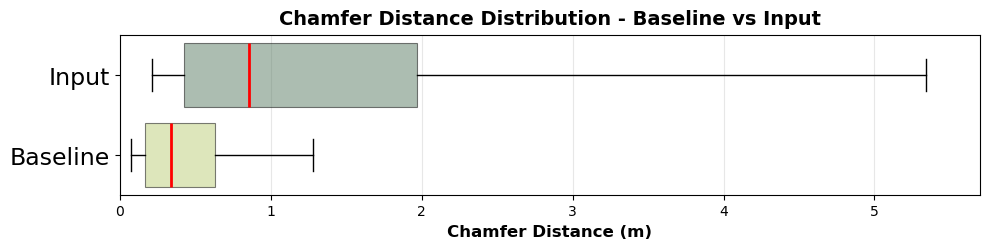
\includegraphics[width=0.9\linewidth]{manuscript/figures/baseline_v_input_boxplot.png}
    \caption{Distribution of Chamfer distance (CD) reconstruction errors comparing raw input data to the 3DEP LiDAR-only baseline model, each evaluated against the reference. Horizontal boxplots show the median (red line), interquartile range (colored boxes), and 10th–90th percentile whiskers; outliers beyond the 90th percentile are excluded. The baseline model shows a lower median CD (0.340 m vs. 0.858 m) with a tighter distribution.\footnote{CD can vary with sampling density and point counts; since the input and predictions (2$\times$ upsampled) differ in size relative to the reference, these magnitudes are not a normalized comparison and are shown for qualitative context \citep{wu2021dcd,lin2023hcd}.}}
    \label{fig:baseline_v_input_boxplot}
\end{figure}

\begin{widefigure}[!t]
    \vspace{-15pt}
    \centering
    \includegraphics[width=1\linewidth]{manuscript/figures/baseline_prediction_example.png}
    \caption{A comparison of baseline (3DEP LiDAR only) model output vs input}
    \label{fig:baseline_pt_cloud_example}
\end{widefigure}

\begin{figure}
    \centering
    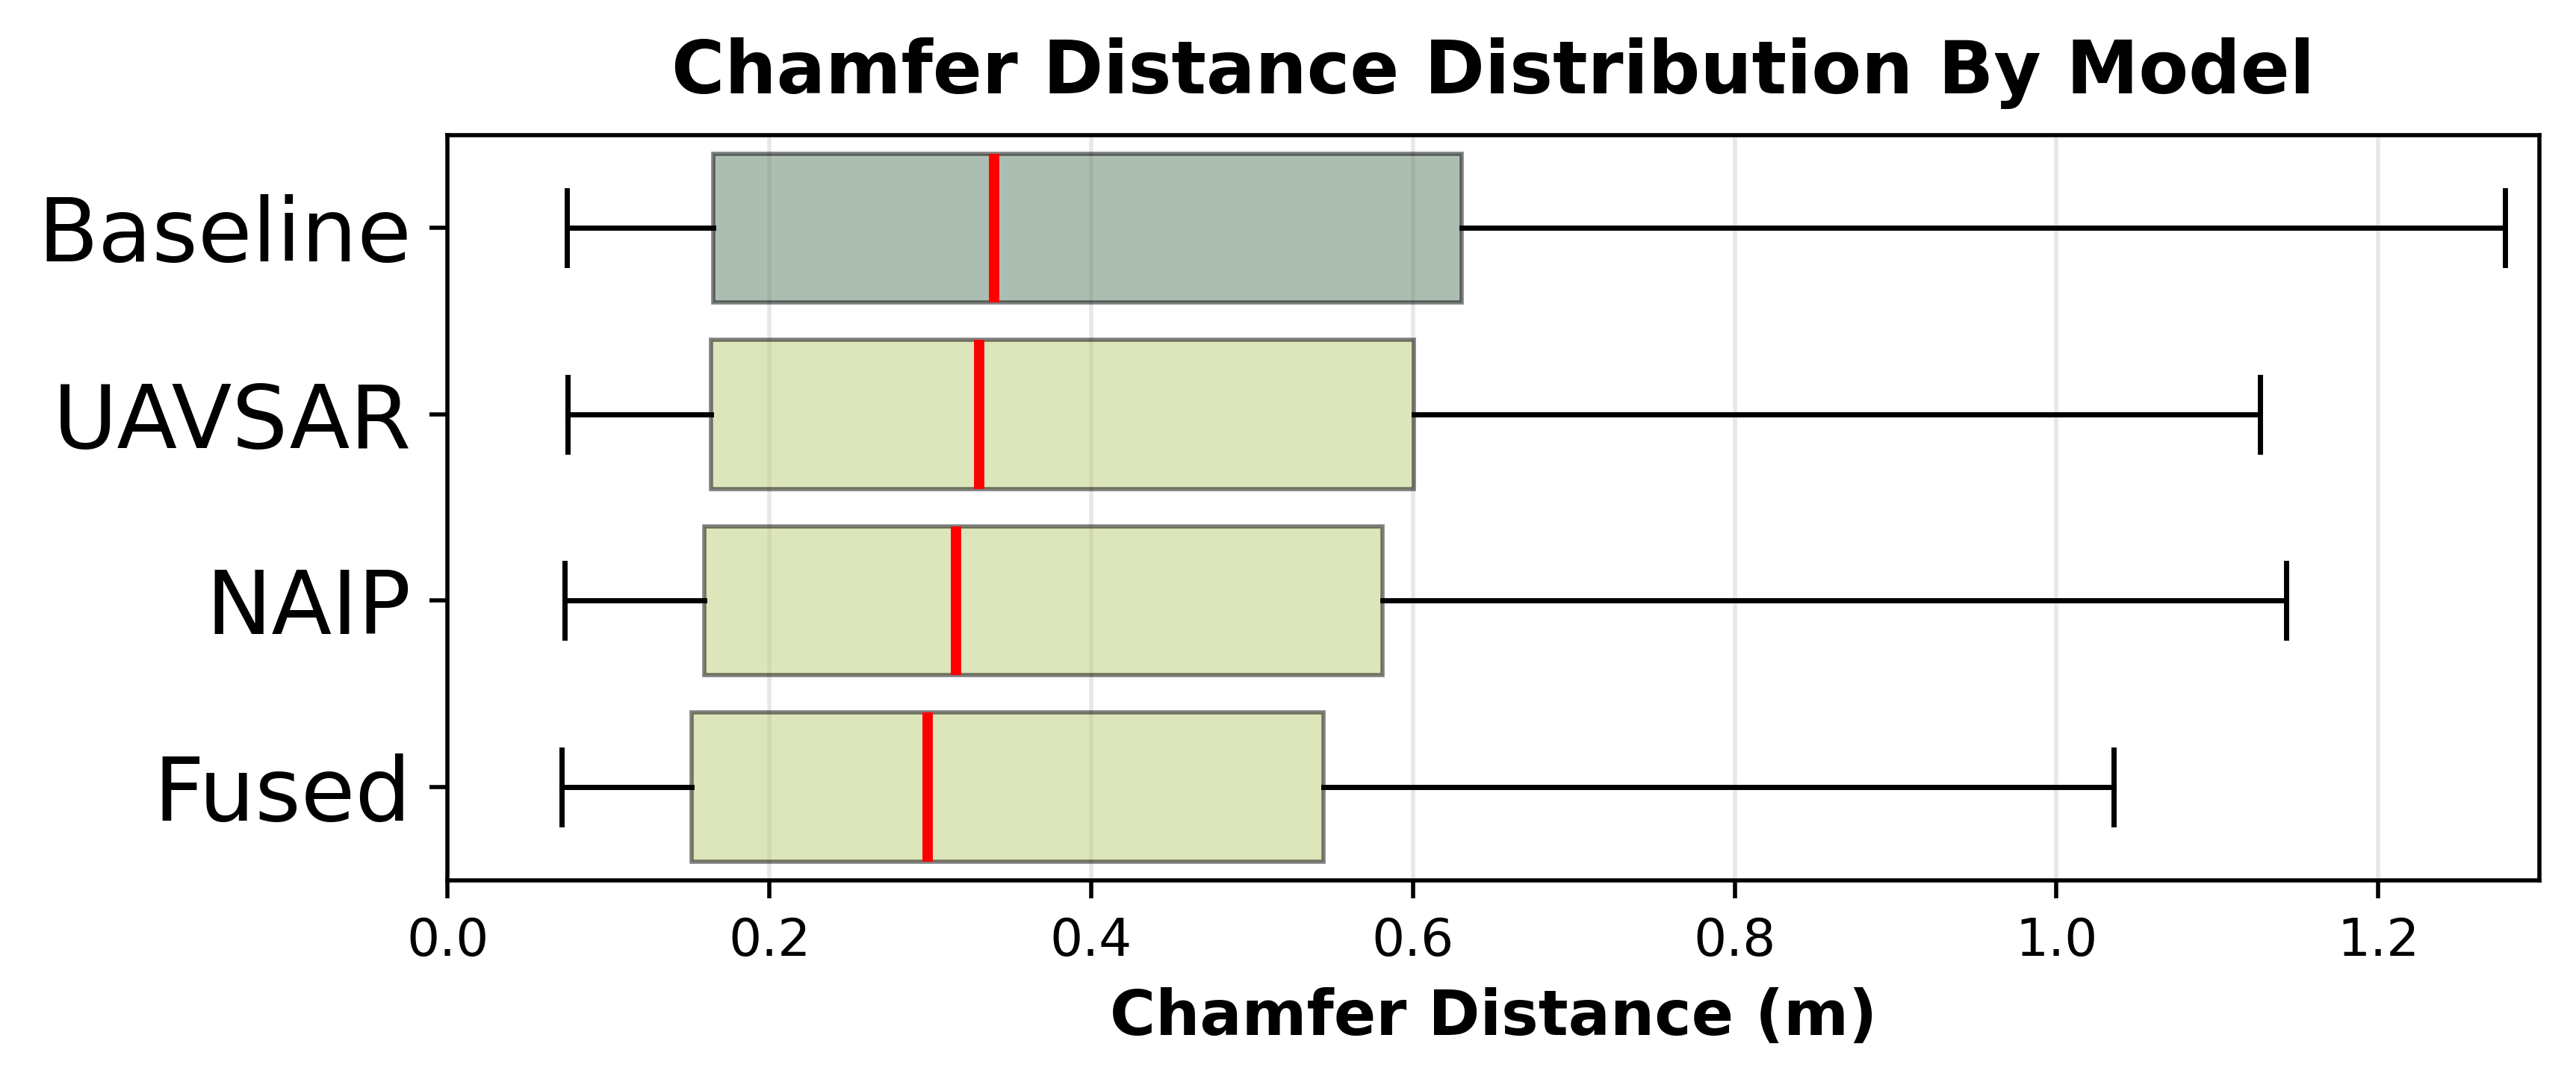
\includegraphics[width=0.75\linewidth]{manuscript/figures/boxplot_by_model.png}
    \caption{Distribution of Chamfer distance reconstruction errors across point cloud upsampling models. Horizontal boxplots show median (red line), interquartile range (colored boxes), and 10th-90th percentile whiskers for models trained with different input modalities. All models demonstrate substantial improvement over the LiDAR-only baseline, with the fused model achieving the lowest median error (0.298 m) and tightest distribution. Outliers beyond the 90th percentile are excluded for clarity.}
    \label{fig:boxplot_model_comparison}
\end{figure}





\begin{table}[htbp]
\centering
\caption{RQ1 \& RQ2: Impact of Single and Fused Modalities on Reconstruction Error}
\label{tab:rq1_rq2_combined}
\begin{tabular}{lcc}
\toprule
\textbf{Comparison} & \textbf{Median Change (\%)} & \textbf{Effect Size} \\
\midrule
\multicolumn{3}{l}{\textit{RQ1: Single Modality vs. Baseline}} \\
\quad NAIP vs Baseline & \textbf{0.5} (p$<$0.001) & \textbf{0.088} \\
\quad UAVSAR vs Baseline & \textbf{0.3} (p$<$0.001) & \textbf{0.062} \\
\midrule
\multicolumn{3}{l}{\textit{RQ2: Fused Modality vs. Best Single Modality}} \\
\quad Fused vs NAIP & \textbf{0.7} (p$<$0.001) & \textbf{0.133} \\
\bottomrule
\end{tabular}
\end{table}




\begin{widefigure}
    \vspace{-20pt}
    \centering
    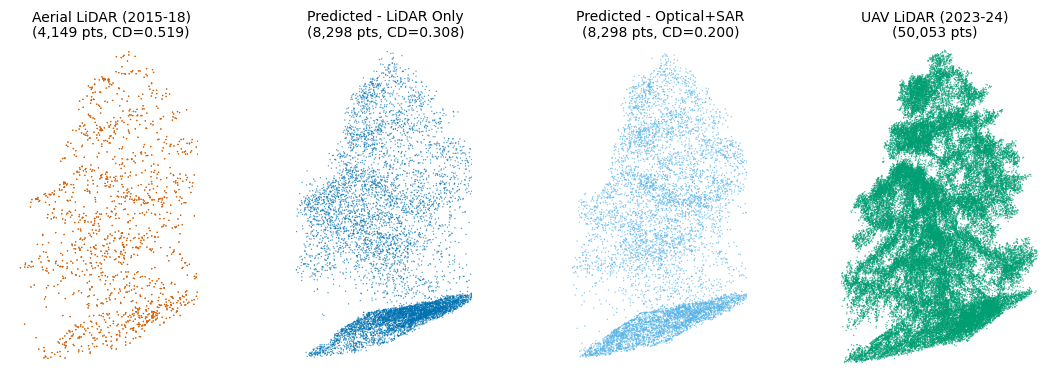
\includegraphics[width=1\linewidth]{manuscript/figures/model_output_example.png}
    \caption{Example tile where no major vegetation change occurred between the 3DEP aerial LiDAR (2015--2018) and UAV LiDAR (2023--2024). The optical+SAR fusion model more accurately recovers fine-scale canopy structure compared to the LiDAR-only model, producing a point cloud that more closely matches the UAV LiDAR reference (lower Chamfer Distance).}
    \label{fig:model_output_example}
\end{widefigure}


Both high-resolution optical imagery (NAIP) and L-band SAR imagery significantly reduced reconstruction error compared to the LiDAR-only baseline, with optical imagery providing slightly larger improvements (0.5\% vs 0.3\%). While statistically significant, the modest effect sizes (0.088 and 0.062 respectively) suggests that single-modality improvements over the baseline upsampling approach are limited in magnitude or may be concentrated in a limited number of tiles. Next, to evaluate our second research question (RQ2), we assessed whether fusing both imagery types yielded additional benefits over the best single-modality model (Table \ref{tab:rq1_rq2_combined}).


The fusion of both optical and SAR imagery yielded additional reconstruction accuracy gains (0.7\% median reduction) beyond using NAIP alone, with a stronger effect size (0.133) than either individual modality achieved in RQ1. This statistically significant improvement supports our hypothesis that the two modalities contain complementary information that can be effectively combined through attention-based fusion. The results demonstrate that multi-modality approaches can leverage different sensing capabilities to achieve superior point cloud reconstruction (Figure \ref{fig:model_output_example}).

Finally, to evaluate our third research question (RQ3) on the impact of vegetation change, we correlated model error with the magnitude of canopy height changes between the legacy 3DEP and recent UAV LiDAR surveys. Table \ref{tab:rq3_results} shows the overall Spearman rank correlations. To investigate this relationship further, we split the dataset into areas of net canopy gain and net canopy loss, with the results of this extended analysis presented in Table \ref{tab:rq3_extended_results}.

\begin{table}[htbp]
\centering
\caption{RQ3: Correlation Between Reconstruction Error and Canopy Height Change}
\begin{tabular}{lcc}
\toprule
\textbf{Model} & \textbf{Spearman $\rho$} & \textbf{p-value} \\
\midrule
Baseline & \textbf{0.650} & p$<$0.001 \\
NAIP & \textbf{0.612} & p$<$0.001 \\
UAVSAR & \textbf{0.628} & p$<$0.001 \\
Fused & \textbf{0.582} & p$<$0.001 \\
\midrule
Baseline vs NAIP (z) & \textbf{3.377} & p$<$0.001 \\
Baseline vs UAVSAR (z) & \textbf{1.999} & p=0.046 \\
Baseline vs Fused (z) & \textbf{5.868} & p$<$0.001 \\
\bottomrule
\end{tabular}
\label{tab:rq3_results}
\end{table}


\begin{table}[htbp]
\centering
\caption{RQ3 Extended: Correlation Between Reconstruction Error and Canopy Height Changes (Gains vs. Losses)}
\begin{tabular}{lcccc}
\toprule
\multirow{2}{*}{\textbf{Model}} & \multicolumn{2}{c}{\textbf{Canopy Gains (N=2423)}} & \multicolumn{2}{c}{\textbf{Canopy Losses (N=3264)}} \\
\cmidrule(lr){2-3} \cmidrule(lr){4-5}
 & \textbf{Spearman $\rho$} & \textbf{p-value} & \textbf{Spearman $\rho$} & \textbf{p-value} \\
\midrule
Baseline & \textbf{0.601} & p$<$0.001 & \textbf{0.671} & p$<$0.001 \\
Naip & \textbf{0.586} & p$<$0.001 & \textbf{0.621} & p$<$0.001 \\
Uavsar & \textbf{0.597} & p$<$0.001 & \textbf{0.637} & p$<$0.001 \\
Fused & \textbf{0.587} & p$<$0.001 & \textbf{0.580} & p$<$0.001 \\
\midrule
Baseline vs Naip (z) & 0.825 & p=0.409 & \textbf{3.440} & p$<$0.001 \\
Baseline vs Uavsar (z) & 0.233 & p=0.816 & \textbf{2.406} & p=0.016 \\
Baseline vs Fused (z) & 0.768 & p=0.442 & \textbf{6.074} & p$<$0.001 \\
\bottomrule
\end{tabular}
\label{tab:rq3_extended_results}
\end{table}


All models showed strong correlations with absolute canopy height change, confirming that reconstruction error systematically increases with vegetation structure changes since the original LiDAR collection. The baseline model exhibited the strongest correlation with canopy change ($\rho=0.650$), while the fused model showed the weakest ($\rho=0.582$), with this difference being statistically significant ($z=5.868$, $p<0.001$). Importantly, the extended analysis revealed this pattern was driven primarily by canopy losses, where the baseline model performed significantly worse than all other models, particularly the fusion approach ($z=6.074$, $p<0.001$), while for canopy gains, all models performed similarly without statistically significant differences. These findings partially support our hypothesis that advanced models better mitigate error from canopy changes, but specifically for canopy removal scenarios where legacy LiDAR contains no information about the removed vegetation (Figures \ref{fig:single_veg_loss_example} and \ref{fig:error_vs_cnpy_chng}). For canopy gains the limited separation is consistent with our original reasoning: most growth cases represent incremental vertical or volumetric accretion within an existing structural envelope already partly encoded in the sparse legacy LiDAR, allowing even the baseline to extrapolate plausibly. Ancillary optical and SAR cues add comparatively little discriminative signal for these modest positive changes, whereas abrupt canopy removal creates a true information void that fused imagery helps fill.

\begin{widefigure}
    \centering
    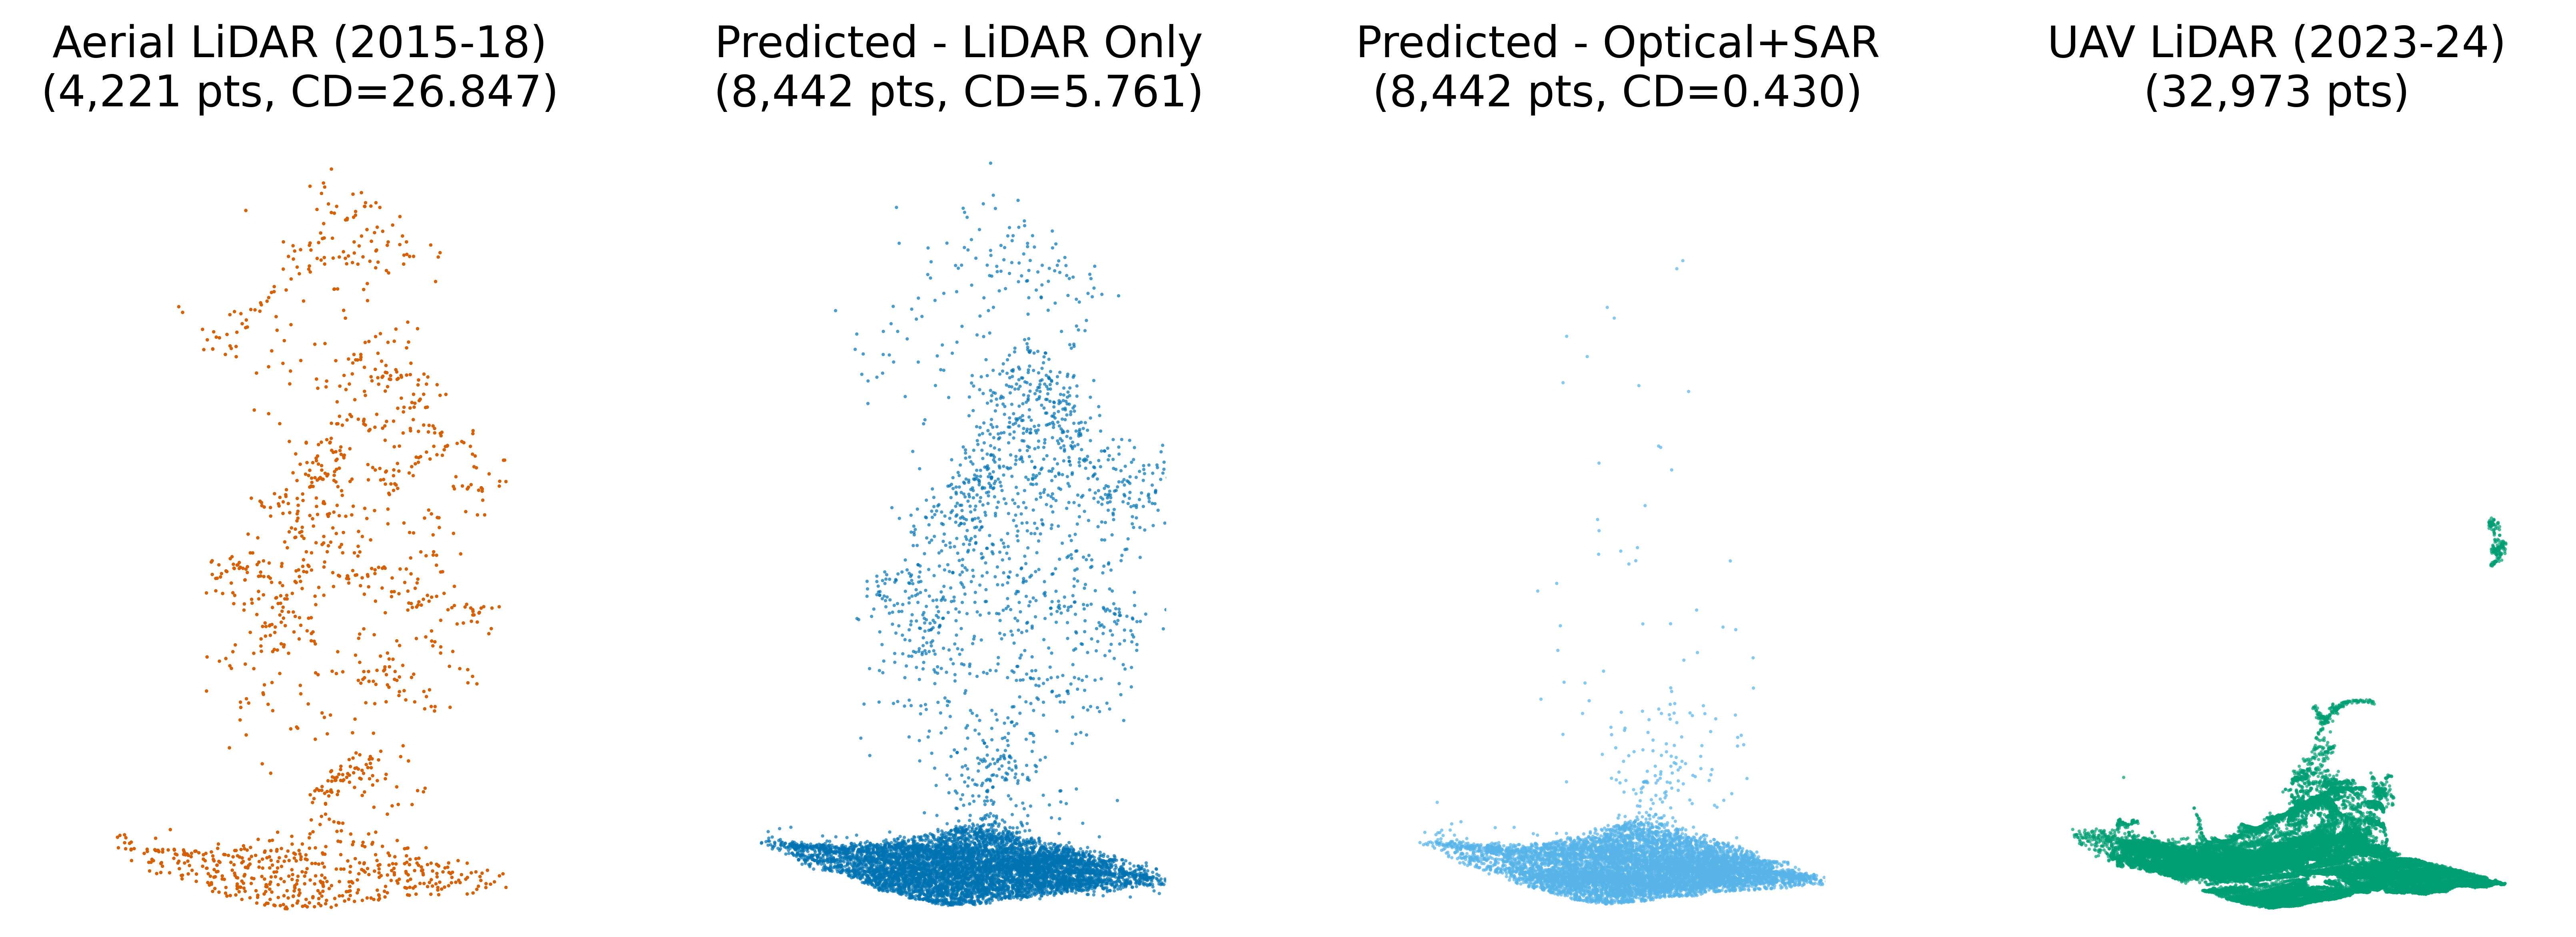
\includegraphics[width=1\linewidth]{manuscript/figures/single_veg_loss_example.png}
    \caption{Example tile illustrating vegetation structure change between legacy aerial LiDAR (2015--2018) and recent UAV LiDAR (2023--2024). The optical+SAR fusion model accurately reconstructs the canopy loss visible in the UAV LiDAR reference, whereas the LiDAR-only model retains outdated structure from the earlier survey. This highlights the value of multi-modal imagery in correcting legacy LiDAR and detecting structural change.}
    \label{fig:single_veg_loss_example}
\end{widefigure}

\begin{widefigure}
    \vspace{-20pt}
    \centering
    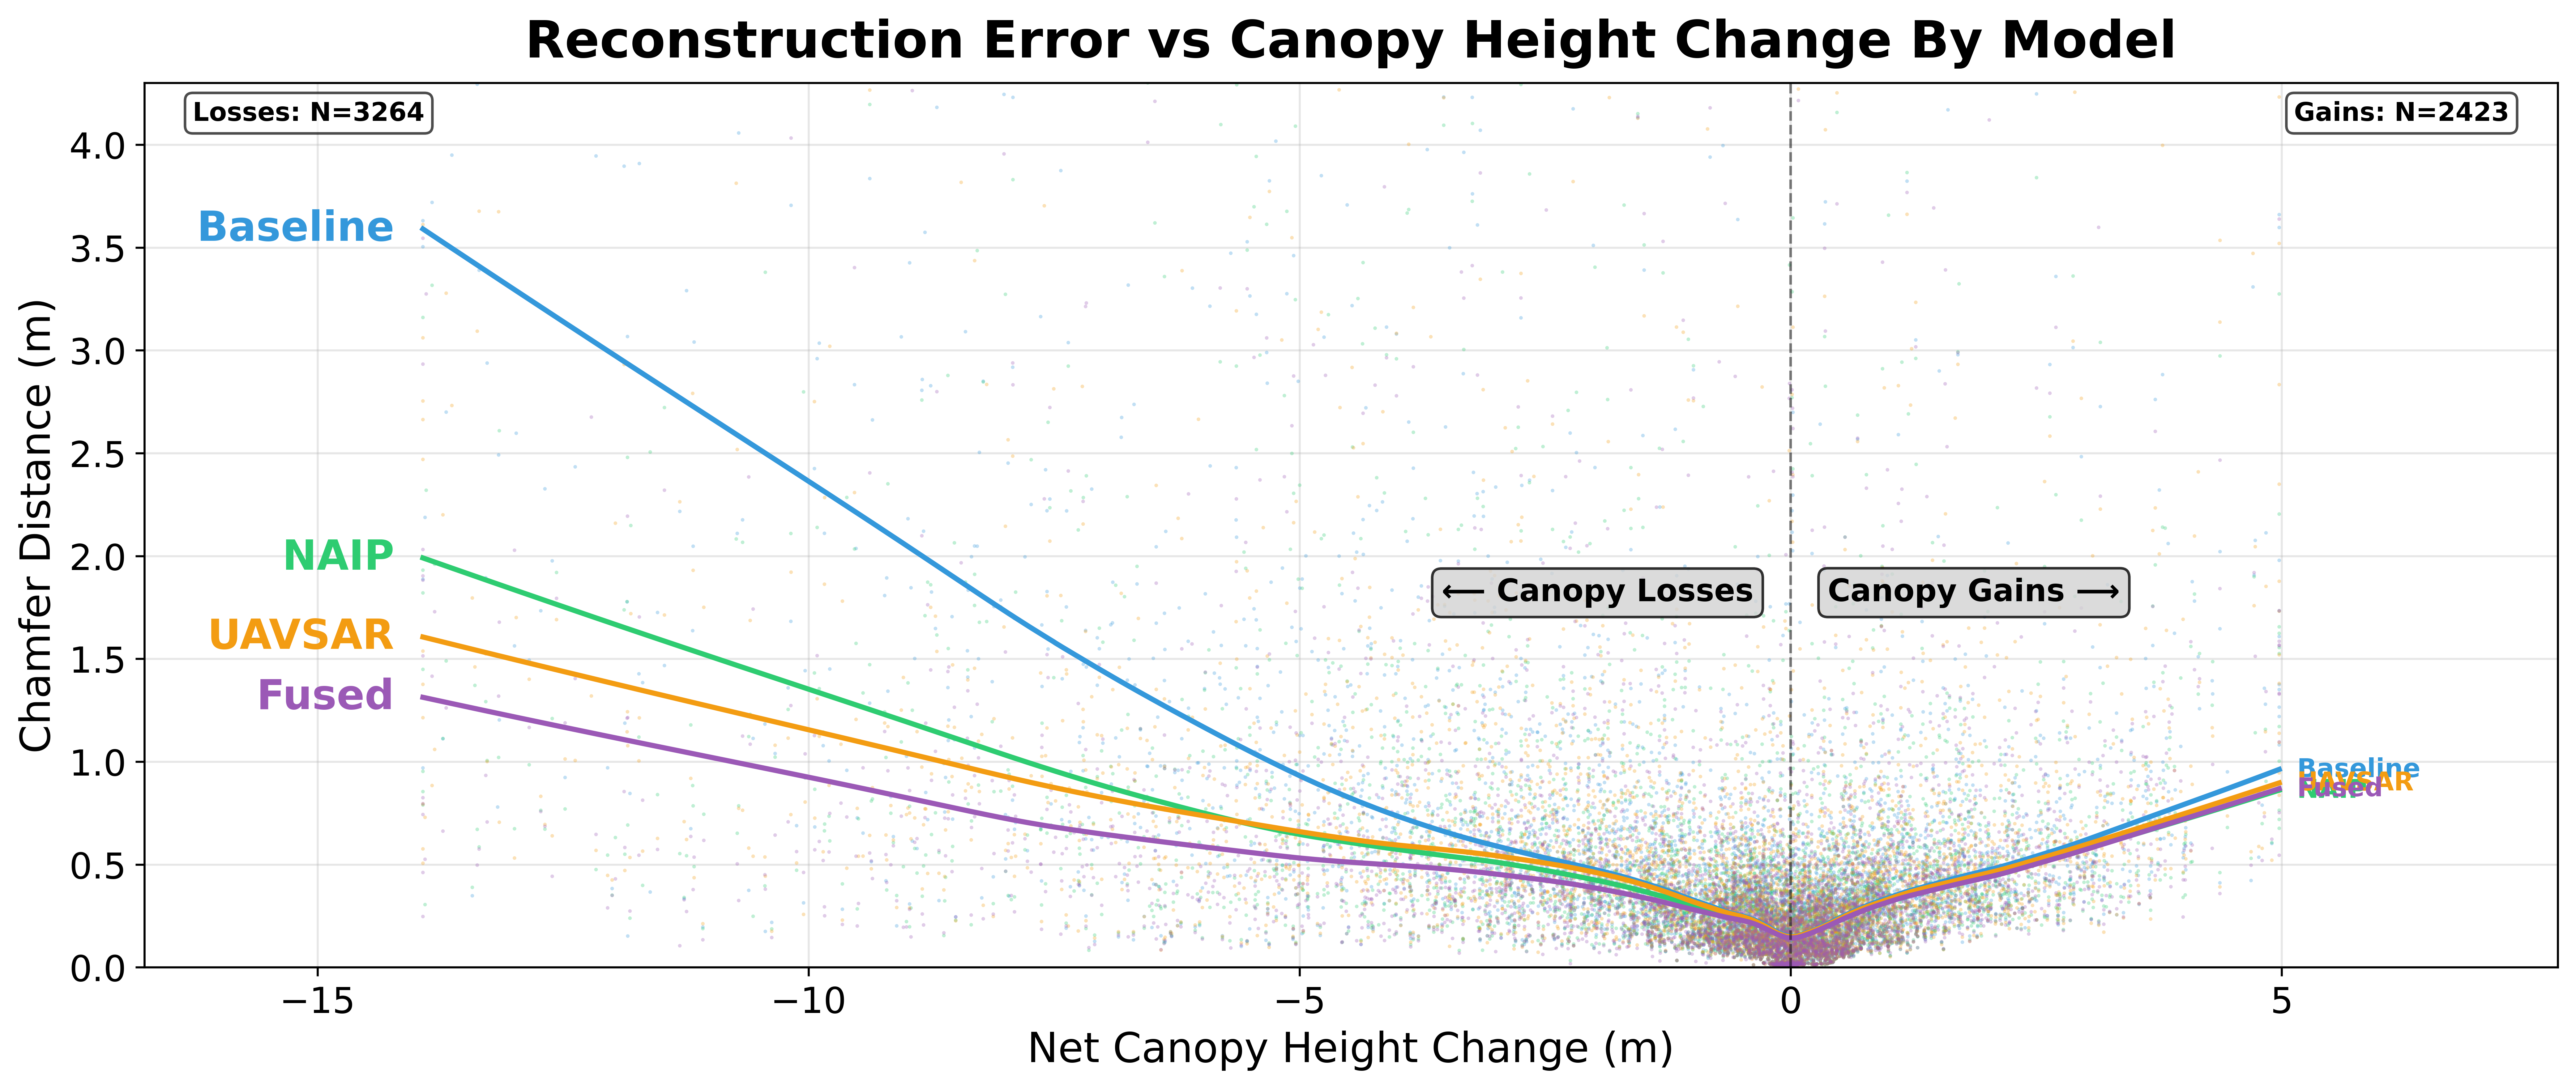
\includegraphics[width=1\linewidth]{manuscript/figures/error_vs_cnpy_chng.png}
    \caption{Relationship between point cloud reconstruction error (Chamfer distance) and net canopy height change since the original LiDAR survey. Scatter points show individual sample tiles (N=5,687) with LOWESS trend lines for each model; outliers above the 99.5th percentile for both error and height change metrics were excluded for visualization clarity. Negative values represent canopy losses while positive values represent gains. The baseline model (blue) shows substantially higher error rates for large canopy losses compared to models incorporating additional remote sensing data (NAIP optical, UAVSAR radar, and fused approaches), while all models perform similarly for canopy gains.}
    \label{fig:error_vs_cnpy_chng}
\end{widefigure}

%%%%%%%%%%%%%%%%%%%%%%%%%%%%%%%%%%%%%%%%%%
\section{Discussion}



This study demonstrates the significant potential of attention-based deep learning models to enhance sparse and outdated airborne LiDAR point clouds by fusing them with more frequently acquired optical (NAIP) and Synthetic Aperture Radar (UAVSAR) imagery. Our findings directly address the critical need for up-to-date, high-resolution 3D vegetation structure information in applications like wildfire risk modeling and ecological monitoring.

The core success of our approach lies in the effective fusion of multi-modal data. As hypothesized (RQ1), both NAIP optical imagery and L-band UAVSAR imagery, when individually integrated, improved point cloud reconstruction accuracy compared to a baseline model relying solely on sparse LiDAR. NAIP, with its finer spatial resolution, offered a slightly greater enhancement, likely due to its ability to delineate canopy edges and small gaps with high fidelity. However, the true advancement was observed when these modalities were combined (RQ2). The fused model, leveraging both NAIP's textural detail and UAVSAR's structural sensitivity, outperformed single-modality enhancements. This confirms our hypothesis that these sensors provide complementary, rather than redundant, information, and that the cross-attention mechanisms within our architecture can effectively identify and leverage these synergistic relationships. This synergy is particularly valuable for capturing the complex, heterogeneous nature of vegetation.

Our investigation into temporal dynamics (RQ3) revealed that all models, including the baseline, exhibited increased reconstruction error in areas with substantial canopy change since the initial LiDAR survey. This is expected, as the input LiDAR reflects a past state. However, the fused model demonstrated the most robust performance, showing a significantly weaker correlation between error and the magnitude of canopy change, especially in areas of canopy loss. This is a crucial finding: by incorporating more recent imagery, particularly the optical data that clearly depicts vegetation absence, the model can more effectively correct for outdated LiDAR information. The baseline model, lacking this current-state information, struggled most in loss scenarios. Even in areas of canopy growth, while not as pronounced as with loss, the image-informed models offered an advantage by providing cues about new or denser vegetation that the original sparse LiDAR could not capture. This capacity to "update" historical LiDAR datasets significantly enhances their utility for long-term monitoring and management, especially in landscapes prone to rapid changes from disturbances or growth.

The developed Local-Global Point Attention Block (LG-PAB) proved to be a robust architectural component. Its ability to capture both fine-grained local details through neighborhood-level self-attention and broader structural coherence via global attention across the entire point patch is central to its success. This hierarchical attention is well-suited to the fractal-like patterns often observed in natural vegetation.

Despite these promising results, some limitations exist. The improvements, while statistically significant, were modest in terms of percentage change in Chamfer distance. This suggests that while fusion helps, there might be inherent limits to upsampling very sparse LiDAR or that the current metrics may not fully capture all aspects of structural improvement relevant to ecological applications.

We acknowledge that perfect cross-sensor alignment is not guaranteed in practice. We deliberately selected established, well-orthorectified public datasets (3DEP, NAIP, UAVSAR) to minimize gross misregistration, and we chose point-to-image cross-attention (with a modest spatial proximity mask) rather than direct concatenation of co-located patch features partly because attention is more tolerant to small horizontal offsets and timing differences among inputs: it allows each point to attend to the most informative nearby patch rather than a single fixed location. We did not conduct a formal misregistration sensitivity study, which we identify as future work. More broadly, our experiments and training were conducted in Southern California's Mediterranean ecosystems; model performance—and the relative contributions of optical versus radar—may differ in other biomes with distinct vegetation structure and phenology. Accordingly, out-of-domain application without additional high-density LiDAR may degrade performance; however, incorporating UAV LiDAR from new biomes into training is a straightforward path to broader generalization.

Beyond the primary 2x upsampling task, we also conducted a preliminary investigation into the model's potential for higher-ratio densification (8x). This exploratory model was scaled up significantly, with larger feature dimensions (512 point, 192 image), more local attention heads for extraction and expansion (16), and a total of ~125M parameters. With our hardware, this increased model size necessitated reducing the batch size to one per GPU. The results (Figure \ref{fig:upsampling_comparison_8x}) show that the architecture can indeed produce highly dense outputs that qualitatively approach the reference data. The appendix provides further qualitative examples from both the standard 2x and experimental 8x models, illustrating their performance across different vegetation change scenarios (Figures \ref{fig:appendix_growth1}--\ref{fig:appendix_loss}).

\begin{widefigure}[!b]
    \vspace{-10pt}
    \centering
    \includegraphics[width=1\linewidth]{manuscript/figures/example_8x_v_2x.png}
    \caption{Comparison of the standard 2x upsampling model (optical+SAR, 6.8 million parameters) output versus a preliminary high-density 8x model (optical+SAR, 125 million parameters)}
    \label{fig:upsampling_comparison_8x}
\end{widefigure}

A recommended area for future research involves adapting the validated multi-modal feature extraction pipeline for direct prediction of key vegetation structure rasters, such as Canopy Height Models (CHM), canopy cover, Above-Ground Biomass (AGB), and fuel types. Such an adaptation would entail replacing the current point cloud generation head with task-specific regression or classification heads, potentially broadening the practical applicability of this work. Integrating geometric priors, like Digital Surface Models (DSMs) and Digital Terrain Models (DTMs), into the loss function also represents a valuable direction. This could not only enforce greater structural realism but also enable the calculation of reconstruction error at various canopy strata, offering deeper insights into model performance. Furthermore, fine-tuning emerging foundation-model vision transformers, such as the Clay model \cite{clay_model_v1p5}, as shared encoders for NAIP and UAVSAR imagery, warrants exploration to leverage large-scale pretraining for enhanced feature representation. Complementary investigations could include a thorough evaluation of the UAVSAR encoder, particularly optimizing multi-look fusion beyond simple averaging and assessing resampling impacts, alongside ablation studies on the LG-PAB and imagery encoders to pinpoint key architectural contributions and guide further optimization. Future architectural research could also explore simplifying the Local-Global Point Attention Block into a pure Point Attention Block by replacing the k-NN local attention with a global attention module. For greater scalability, this could be paired with a latent attention strategy \cite{liu2024deepseek} to bypass the quadratic complexity inherent to self-attention.


%%%%%%%%%%%%%%%%%%%%%%%%%%%%%%%%%%%%%%%%%%
\section{Conclusions}

This research successfully demonstrates that attention-based deep learning, leveraging our novel Local-Global Point Attention Block, can significantly enhance sparse airborne LiDAR point clouds in vegetated landscapes through the fusion of more recent optical and radar imagery. We have shown that while individual imagery modalities provide benefits, their combined use yields superior reconstruction accuracy, particularly in mitigating errors arising from vegetation changes over time. Specifically, high-resolution optical imagery (NAIP) proved slightly more effective as a standalone ancillary dataset than L-band SAR within our framework, but the fusion of both offered the best performance, validating the complementary nature of these sensors. A key contribution is the model's ability to substantially reduce reconstruction degradation in areas of vegetation loss, thereby increasing the utility of historical LiDAR archives. This study presents a novel approach to direct 3D point cloud upsampling using multi-modal fusion in complex natural environments, moving beyond prevalent raster-based enhancement techniques and paving the way for more accurate and timely assessments of vegetation structure.
%%%%%%%%%%%%%%%%%%%%%%%%%%%%%%%%%%%%%%%%%%


%%%%%%%%%%%%%%%%%%%%%%%%%%%%%%%%%%%%%%%%%%
% \vspace{6pt}

%%%%%%%%%%%%%%%%%%%%%%%%%%%%%%%%%%%%%%%%%%

\authorcontributions{Conceptualization, M.M. and D.S.; methodology, M.M.; software, M.M.; validation, M.M.; formal analysis, M.M.; investigation, M.M. and D.S.; resources, D.S. and J.F.; data curation, M.M.; writing---original draft preparation, M.M.; writing---review and editing, D.S. and J.F.; visualization, M.M.; supervision, D.S. and J.F.; project administration, D.S. and J.F.; funding acquisition, D.S. and J.F. All authors have read and agreed to the published version of the manuscript.}

\funding{Funding for the research was provided by California Climate Action Matching Grants University of California Office of the President grant (\#R02CM708) to M. Jennings, SDSU (PI) and JF. DS gratefully acknowledges funding from the NASA FireSense program (Grant \# 80NSSC24K0145), the NASA FireSense Implementation Team (Grants \#80NSSC24K1320),the NASA Land-Cover/Land Use Change program (Grant \#NNH21ZDA001N-LCLUC), the EMIT Science and Applications Team program (Grant \#80NSSC24K0861), the NASA Remote Sensing of Water Quality program (Grant \#80NSSC22K0907), the NASA Applications-Oriented Augmentations for Research and Analysis Program (Grant \#80NSSC23K1460), the NASA Commercial Smallsat Data Analysis Program (Grant \#80NSSC24K0052), the USDA NIFA Sustainable Agroecosystems program (Grant \#2022-67019-36397), the USDA AFRI Rapid Response to Extreme Weather Events Across Food and Agricultural Systems program (Grant \#2023-68016-40683), the California Climate Action Seed Award Program, and the NSF Signals in the Soil program (Award \#2226649).}




\dataavailability{All Python code used for data collection, preprocessing, model training, and analysis is publicly available on GitHub at \url{https://github.com/mmarks13/geoai_veg_map}. The 3DEP airborne LiDAR and NAIP optical imagery used as model inputs were sourced via Microsoft's Planetary Computer (\url{https://planetarycomputer.microsoft.com/}) using the provided code. The UAVSAR radar imagery was sourced via the Alaska Satellite Facility (\url{https://search.asf.alaska.edu/}) using the provided code. The UAV LiDAR point clouds used as reference data for model training and evaluation are being made available through OpenTopography (\url{https://opentopography.org/}); specific DOIs will be provided upon acceptance or can be requested from the authors. The exact data stacks (input features and reference point clouds) used for model training and evaluation are available from the corresponding author upon reasonable request.}


\acknowledgments{The authors wish to express their sincere gratitude to Lloyd L. ("Pete") Coulter (Center for Earth Systems Analysis Research, Department of Geography, SDSU) for his skillful piloting and management of all UAV LiDAR data acquisition campaigns; this data was foundational to the research presented. Separately, during the preparation of this manuscript, generative AI models (including Google's Gemini, Anthropic's Claude, and OpenAI's ChatGPT) were utilized to assist with language refinement, conceptual brainstorming, generating preliminary code structures, and code debugging. The authors have reviewed and edited all AI-generated suggestions and take full responsibility for the content of this publication.}

\conflictsofinterest{The authors declare no conflicts of interest. The funders had no role in the design of the study; in the collection, analyses, or interpretation of data; in the writing of the manuscript; or in the decision to publish the results}

%%%%%%%%%%%%%%%%%%%%%%%%%%%%%%%%%%%%%%%%%%
%% Optional



\abbreviations{Abbreviations}{
The following abbreviations are used in this manuscript:\\

\noindent
\begin{tabular}{@{}ll}
3DEP & 3D Elevation Program \\
C-ALS & Crewed Airborne LiDAR \\
CAD & Computer-Aided Design \\
CD & Chamfer Distance \\
DSM & Digital Surface Model \\
FFN & Feed-Forward Network \\
GSD & Ground-Sample Distance \\
GRU & Gated Recurrent Unit \\
LG-PAB & Local-Global Point Attention Block \\
LiDAR & Light Detection and Ranging \\
MLP & Multi-Layer Perceptron \\
NAIP & National Agriculture Imagery Program \\
RQ1 & Research Question 1 \\
SAR & Synthetic Aperture Radar \\
UAV & Unmanned Aerial Vehicle \\
UAVSAR & Uninhabited Aerial Vehicle Synthetic Aperture Radar \\
USGS & U.S. Geological Survey \\
ViT & Vision Transformer \\
\end{tabular}
}



% %\isPreprints{}{% This command is only used for ``preprints''.
% \begin{adjustwidth}{-\extralength}{0cm}
% %} % If the paper is ``preprints'', please uncomment this parenthesis.
% %\printendnotes[custom] % Un-comment to print a list of endnotes

% \reftitle{References}

% % Please provide either the correct journal abbreviation (e.g. according to the “List of Title Word Abbreviations” http://www.issn.org/services/online-services/access-to-the-ltwa/) or the full name of the journal.
% % Citations and References in Supplementary files are permitted provided that they also appear in the reference list here.

% %=====================================
% % References, variant A: external bibliography
% %=====================================
% \bibliography{manuscript/references}

% \PublishersNote{}
% %\isPreprints{}{% This command is only used for ``preprints''.
% \end{adjustwidth}
% %} % If the paper is ``preprints'', please uncomment this parenthesis.


\isPreprints{
  % This code runs ONLY if it IS a preprint
  \begin{adjustwidth}{-\extralength}{0cm}
  \reftitle{References}
  \bibliography{manuscript/references}
  \PublishersNote{}
  \end{adjustwidth}
}{
  % This code runs ONLY if it is NOT a preprint
  \reftitle{References}
  \bibliography{manuscript/references}
  \PublishersNote{}
}
%%%%%%%%%%%%%%%%%%%%%%%%%%%%%%%%%%%%%%%%%%
%% Optional
\clearpage
\appendixtitles{no} % Leave argument "no" if all appendix headings stay EMPTY (then no dot is printed after "Appendix A"). If the appendix sections contain a heading then change the argument to "yes".
\appendixstart
\appendix
% Appendix visualization note (Reviewer 1 Fig A3 concern)
\begin{table}[H]
  \centering
  \caption{Detailed layer specifications not fully enumerated in the main text. All experiments use $D_{\text{p\_feat}}=256$, $D_{\text{token}}=128$, upsampling ratio $R_{\text{up}}=2$, and KNN $k=16$.}
  \label{tab:layer_specs}
  \small
  \begin{tabular}{p{3.2cm} p{10.8cm}}
    	oprule
    Component & Specification \\
    \midrule
    Patch Conv Stem & Conv1 $C_{in}\rightarrow D_{tok}/2$ ($3\times3$, s=1,p=1) – GELU – Conv2 $D_{tok}/2\rightarrow D_{tok}$ ($3\times3$, s=1,p=1) – AvgPool (k=stride=10) – LayerNorm. \\
    Transformer Encoder MLP & $D_{tok} \rightarrow 4D_{tok}$ – depth-wise 1-D conv (k=3) – GELU – $\rightarrow D_{tok}$ (LayerScale $\gamma\approx10^{-5}$; 4 heads self-attn). \\
    Temporal GRU Head & Bi-GRU hidden=$D_{tok}$ (fwd+bwd) – attention pooling (Linear $2D_{tok}\rightarrow1$). \\
    Cross-Attention Fusion & Point query proj: Linear $256\rightarrow256$; NAIP/UAVSAR key \/ value proj: Linear $(128+pos_{patch})\rightarrow256$ (pos enc dim 24); multi-head (4) scaled dot-product; post-concat MLP: Linear $C\rightarrow C$ – GELU – Linear $C\rightarrow256$ + residual + LayerNorm. \\
    LG-PAB Local Attention & Multi-head PointTransformerConv (4 heads) over KNN graph ($k=16$); per-head out dim $256/4$; FFN after local attn: $256\rightarrow512\rightarrow256$ (GELU). \\
    LG-PAB Global Attention & Position MLP $3\rightarrow32\rightarrow32$; concatenate with features; 4-head global FlashAttention; FFN: $256\rightarrow512\rightarrow256$ (GELU). \\
    Feature-Guided Upsampling & Intermediate reshape $[N,R,256]$; Position-Generator MLP $256\rightarrow64\rightarrow32\rightarrow3$ (GELU); feature clones flattened to $(R\cdot N,256)$. \\
    Coordinate Decoder & MLP $256\rightarrow128\rightarrow64\rightarrow32\rightarrow3$ (GELU) producing residual offsets. \\
    Normalization & LayerNorm after major residual joins (fusion output; after local and global attention outputs). \\
    Dropout & Imagery encoder \/ fusion attention: 0.02–0.10; point global attention: 0.02 (no dropout in local PointTransformerConv). \\
    Positional Encodings & Global point attention position MLP (32 dims); patch sinusoidal encoding dim 24. \\
    Optimizer & ScheduleFreeAdamW (shared across variants; see main text Table~\ref{tab:training_protocol}). \\
    \bottomrule
  \end{tabular}
\end{table}

\noindent\textit{Appendix visualization note:} All quantitative metrics in the manuscript are derived from the production 2$\times$ upsampling models. The two vegetation growth examples below use an experimental 8$\times$ model \emph{only} to improve visual legibility of subtle new canopy structure (higher point density reveals incremental infill); these outputs are illustrative and not part of reported statistics. The vegetation loss example is shown with the production 2$\times$ fusion model to reflect the evaluated configuration.
\begin{widefigure}[H]
    \centering
    \includegraphics[width=1\linewidth]{manuscript/figures/veg_growth_8x.png}
  \caption{Example of vegetation growth reconstruction (experimental 8$\times$ model for illustrative visual clarity only; all reported metrics use the production 2$\times$ model). The model successfully infers new canopy structure (center) that is absent in the input 3DEP LiDAR but present in the recent UAV LiDAR reference.}
    \label{fig:appendix_growth1}
\end{widefigure}

\begin{widefigure}[H]
    \centering
    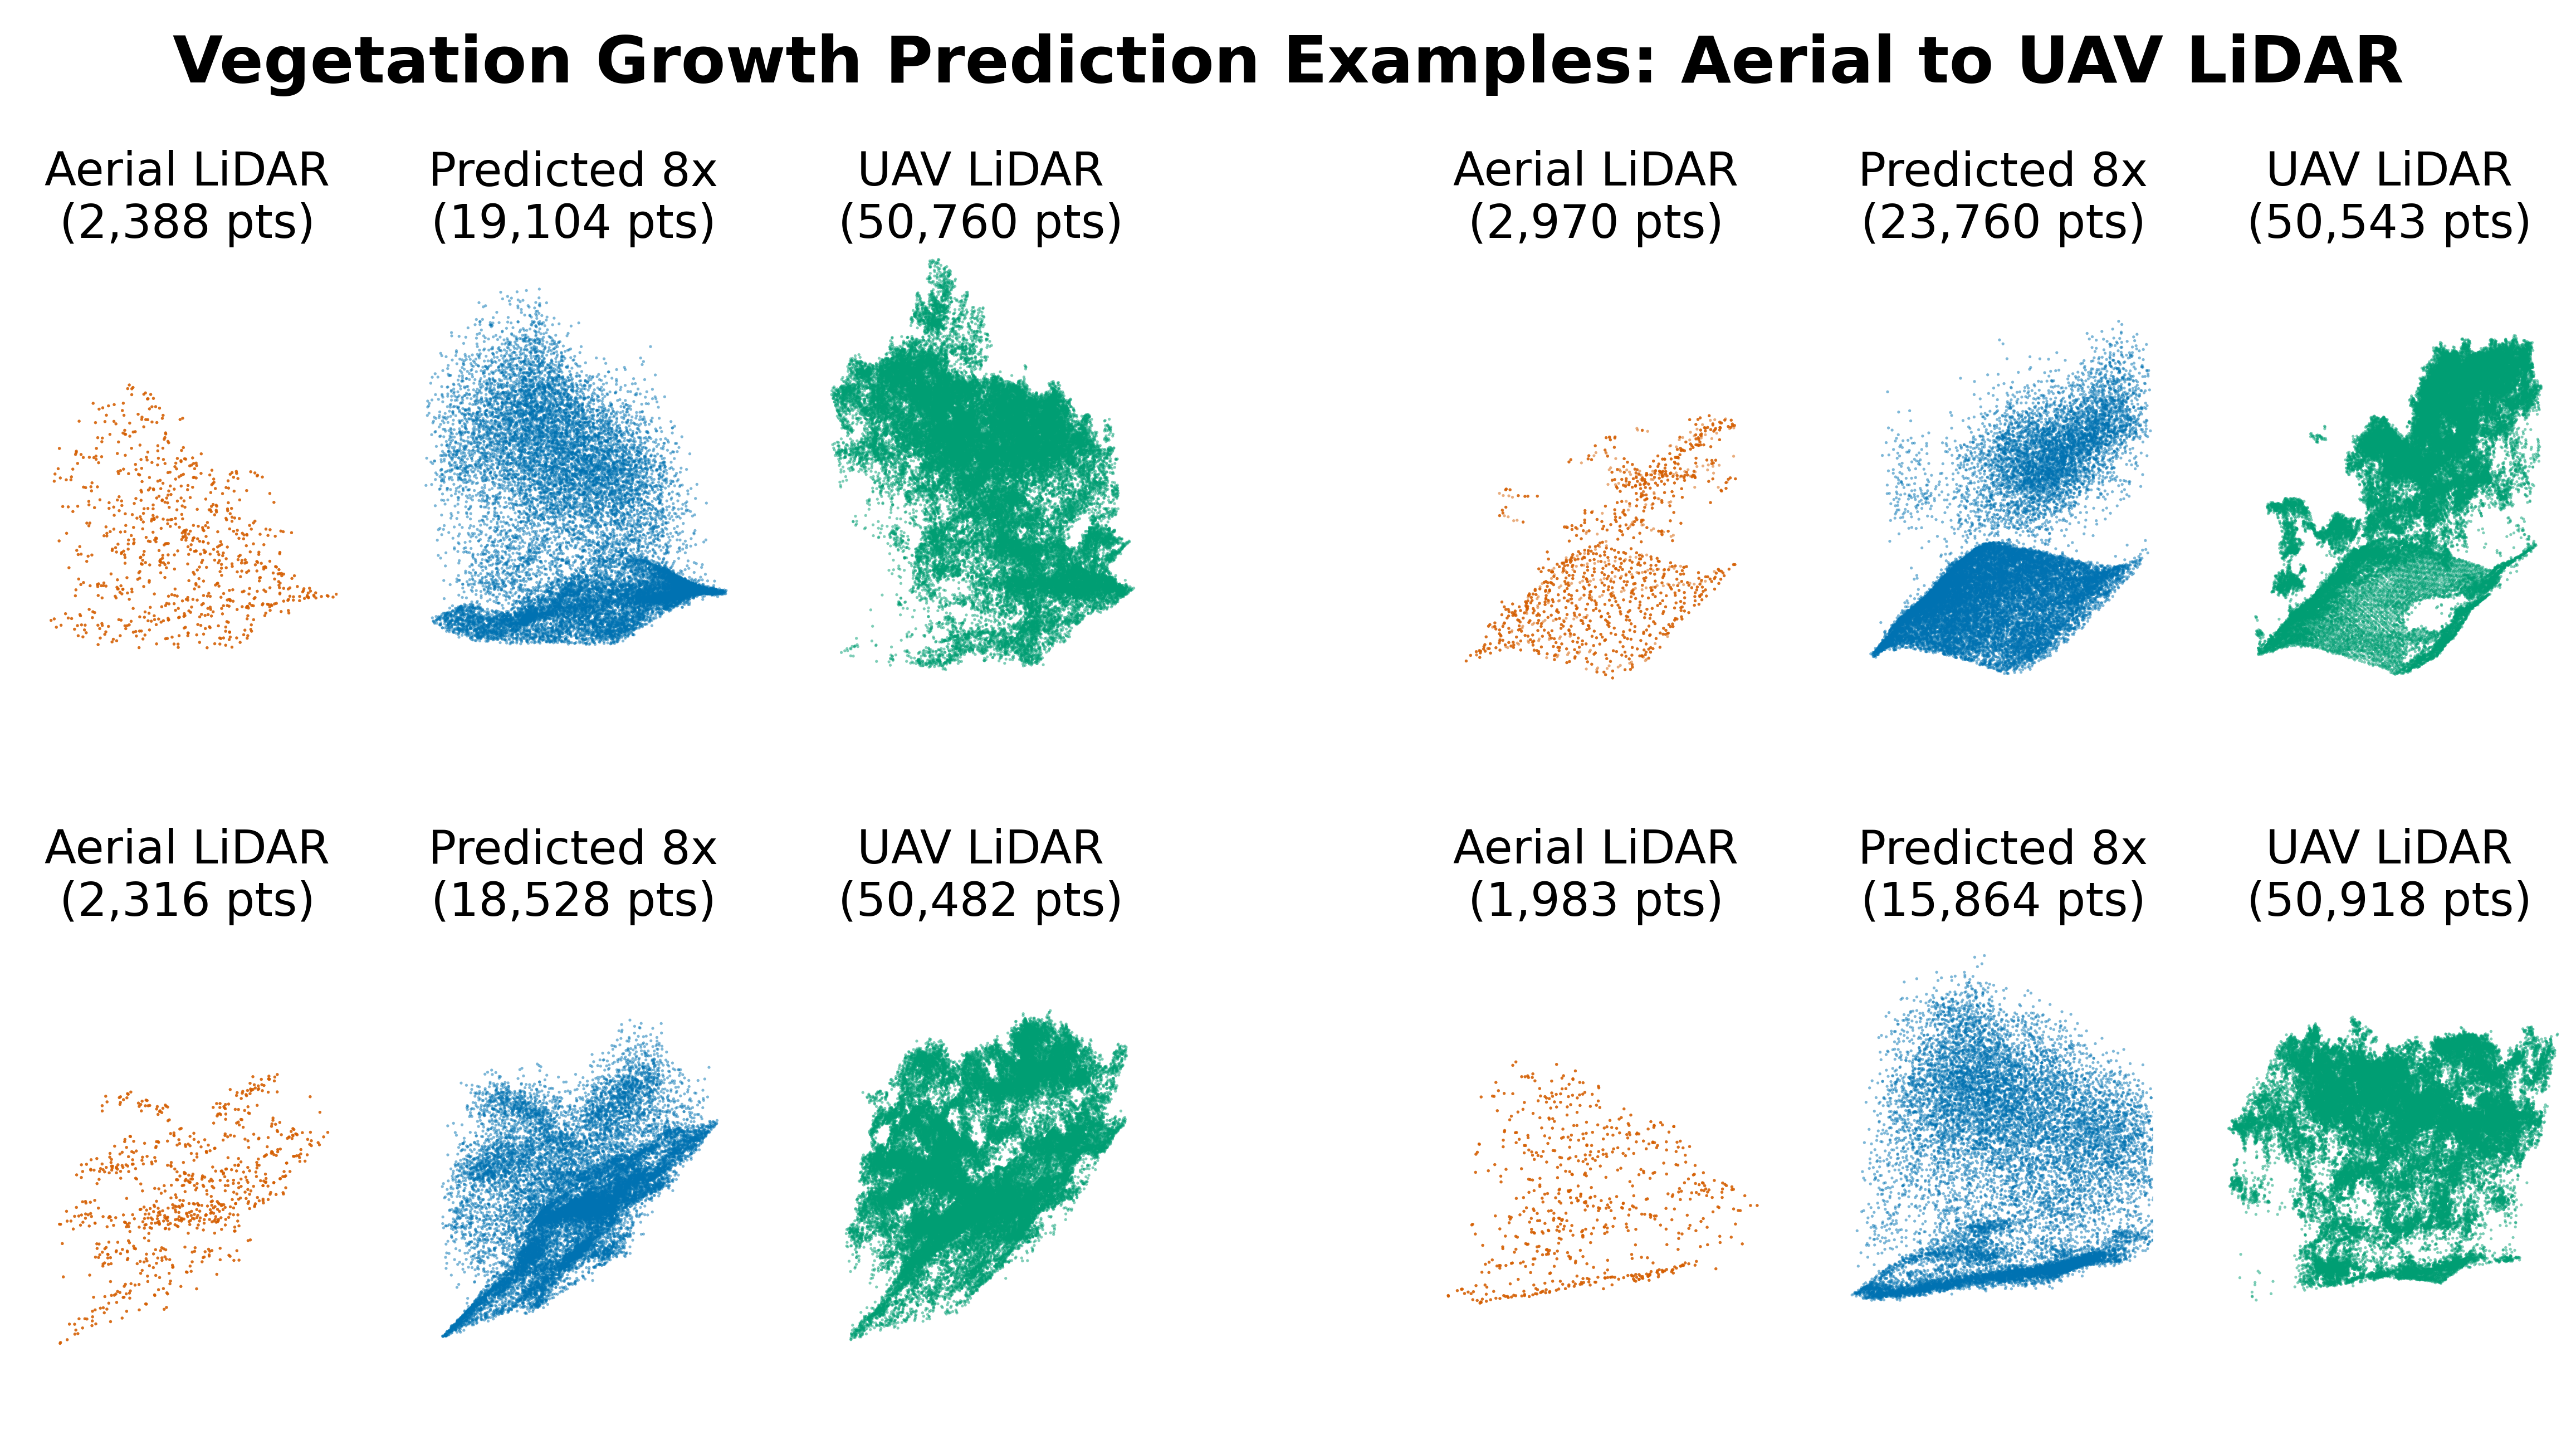
\includegraphics[width=1\linewidth]{manuscript/figures/veg_growth2_8x.png}
  \caption{Second vegetation growth example (experimental 8$\times$ visualization only; quantitative results use the 2$\times$ model).}
    \label{fig:appendix_growth2}
\end{widefigure}

%%%%%%%%%%%%%%%%%%%%%%%%%%%%%%%%%%%%%%%%%%
\begin{widefigure}[H]
    \centering
    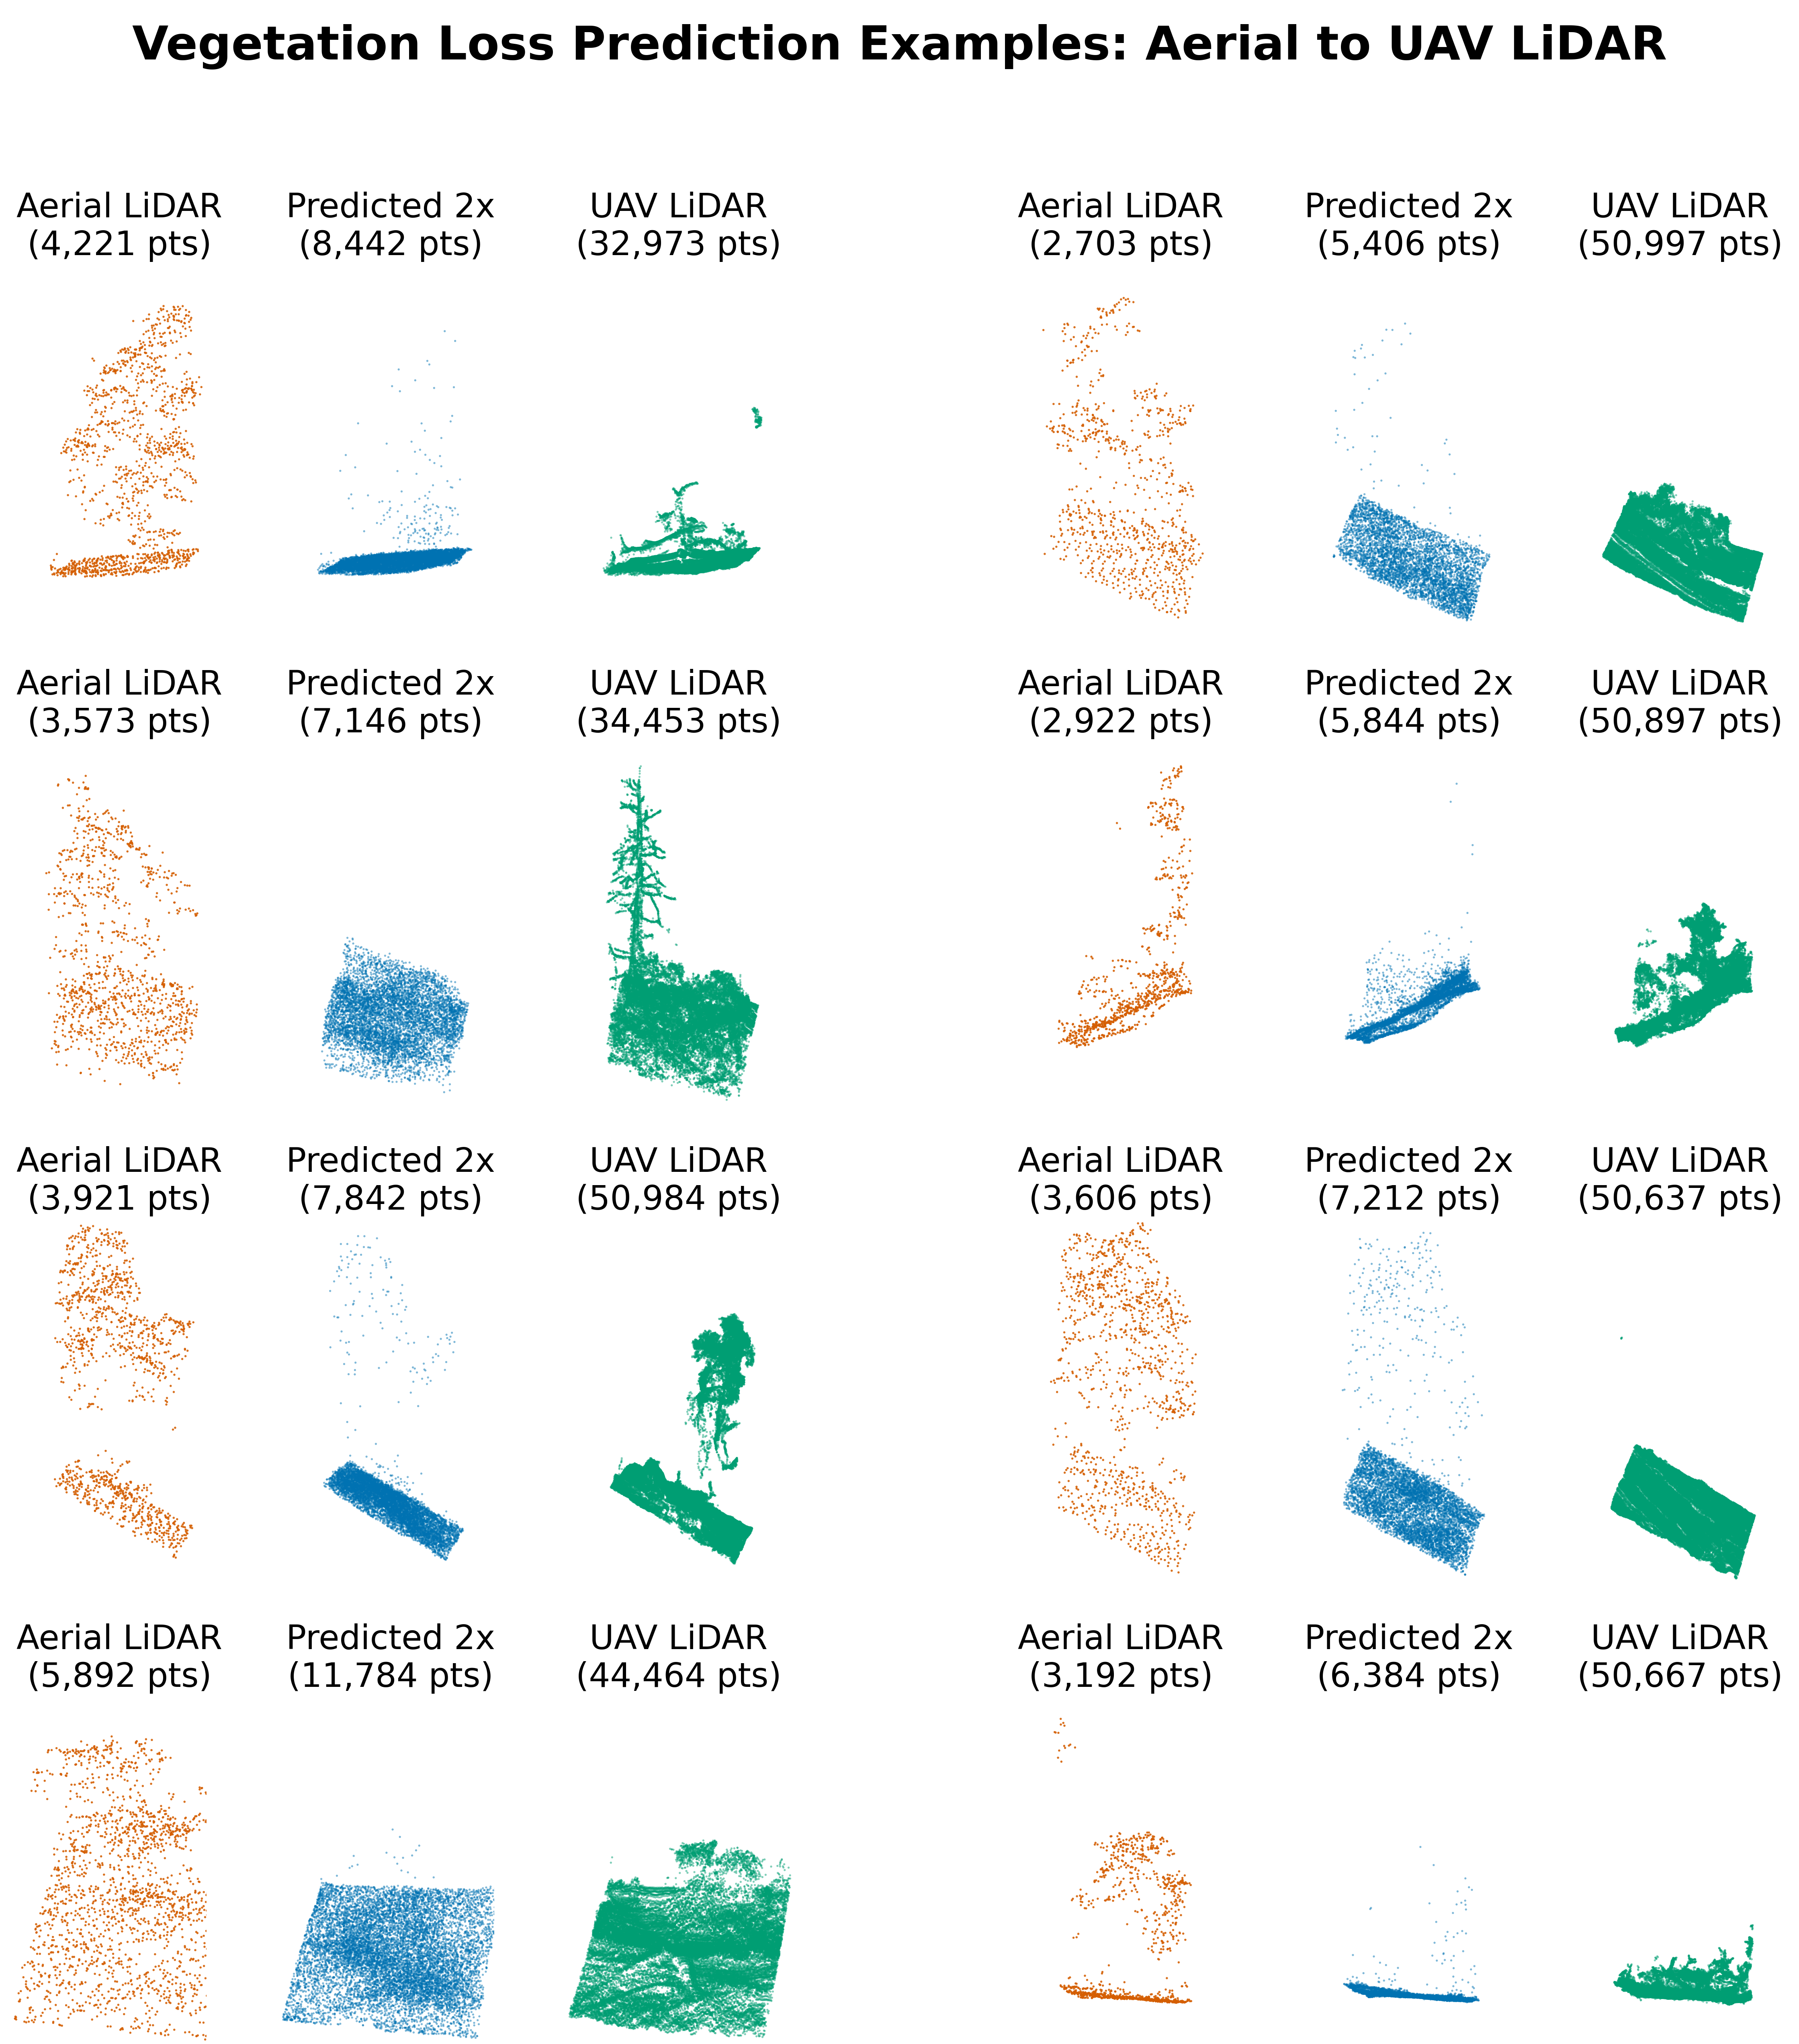
\includegraphics[width=1\linewidth]{manuscript/figures/veg_loss_2x.png}
  \caption{Vegetation loss example using the production 2$\times$ fusion model (configuration used for all quantitative evaluation). The model removes vegetation present in the outdated input LiDAR (left) to match the state shown in the recent UAV LiDAR reference (right), highlighting the value of multi-modal fusion for change detection.}
   \label{fig:appendix_loss}
\end{widefigure}


\end{document}